\documentclass[letter,11pt]{article}

%PACKAGES--------------------------------
%Langue et encodage
\usepackage[english]{babel}
\usepackage[utf8]{inputenc}
\usepackage[T1]{fontenc}
\usepackage{lmodern}
%Gestion de mise en page
\usepackage{supertabular}
%\usepackage{fullpage}
\usepackage{here}% permet, avec [H] de mettre l'image ICI!!! (et pas au petit bonheur la chance LaTeXien)
\usepackage[perpage,symbol]{footmisc} %remet à zéro le compteur des notes de bas de page après chaque page
%\usepackage[hmargin={3cm,3cm}, vmargin={3cm,3cm}, dvips]{geometry}
%\pagestyle{plain}
%\parindent=0cm	%définit la longueur du retrait
%Mathématiques
\usepackage{amsmath} %Formules
\usepackage{amssymb} %Formules
\usepackage{amsthm} %Environnements
%\usepackage{relsize,exscale} %changement taille symboles mathématiques
%\usepackage{amsfonts}
\usepackage{enumerate}
\usepackage{esint}
\usepackage{graphics}
\usepackage{graphicx}
\usepackage{tikz}
%\usepackage{mathrsfs}
%\usepackage{mathtools}
%\usepackage{multirow}
%\usepackage[all]{xy} %xy-pic
%style captions
%\usepackage[font=small,labelfont=bf]{caption}

% pour changer le nom des captions des figures
\usepackage{ccaption}
\addto\captionsfrench{\def\figurename{{Diagramme}}}

%ENVIRONNEMENTS--------------------------
%Définition des styles
\newtheoremstyle{droit}
{}%Space above
{}%Space below
{\upshape}%Body font
{}%Indent amount (empty = no indent, \parindent = para indent)
{\bfseries}%theoreme head font
{}%Punctuation after theoreme head
{ }%{\newline}%Space after theoreme head: " " = normal interword space; \newline = linebreak
{}%theoreme head spec (can be left empty, meaning `normal')
\newtheoremstyle{italique}
{}%Space above
{}%Space below
{\itshape}%Body font
{}%Indent amount (empty = no indent, \parindent = para indent)
{\bfseries}%theoreme head font
{}%Punctuation after theoreme head
{ }%{\newline}%Space after theoreme head: " " = normal interword space; \newline = linebreak
{}%theoreme head spec (can be left empty, meaning `normal')
%Théorèmes
\theoremstyle{italique}
\newtheorem{theorem}{Theorem}[section]
\newtheorem{proposition}[theorem]{Proposition}
\newtheorem{lemma}[theorem]{Lemma}
\newtheorem{corollary}[theorem]{Corollary}
\newtheorem{axiom}[theorem]{Axiom}
\theoremstyle{droit}
\newtheorem{example}[theorem]{Example}
\newtheorem{remark}[theorem]{Remark}
\newtheorem{note}[theorem]{Note}
\newtheorem{definition}[theorem]{Definition}
\newtheorem{notation}[theorem]{Notation}
\newtheorem{terminology}[theorem]{Terminology}
\newtheorem{question}[theorem]{Question}
%Autres
\renewcommand{\thefootnote}{\fnsymbol{footnote}} %dans les notes de bas de page, remplace les chiffres par un symbole
\newenvironment{indice} %comme une liste, mais avec (i), (ii), (iii), (iv)
{\begin{enumerate}[\textup{(}i\textup{)}] }
{\end{enumerate}}
\newenvironment{step}
{\begin{enumerate}[\textup{Step }1\textup{ :}] }
{\end{enumerate}}
\newenvironment{case}
{\begin{enumerate}[\textup{Case } 1\textup{ :}] }
{\end{enumerate}}

%COMMANDES-------------------------------
\newcommand{\N}{\mathbb{N}}
\newcommand{\Z}{\mathbb{Z}}
\newcommand{\Q}{\mathbb{Q}}
\newcommand{\R}{\mathbb{R}}
\newcommand{\C}{\mathbb{C}}
%\newcommand{\L}{\mathcal{L}}
\newcommand{\Ker}{{\rm Ker}}
\newcommand{\Tr}{{\rm Tr}}
\newcommand{\im}{{\rm Im}}
\newcommand{\ch}{{\rm ch}}
\DeclareMathOperator{\spn}{span}
\newcommand{\dans}{\longrightarrow}
\newcommand{\ddans}{\rightrightarrows}
%\newcommand{\tndans}{\Rightarrow}
\newcommand{\Bdot}{\bullet}
\newcommand{\noi}{\noindent}


 

%TITRE-----------------------------------
\title{TODO} %Titre du document
\author{Ondine Chanon and Stefano Savarè} %Auteur du document
\date{Winter 2014}


%DOCUMENT================================
\begin{document}
\begin{titlepage}


\begin{center}
\textsc{Politecnico di Milano - MSc in Mathematical Engineering}

Under the supervision of Prof. M. Verani and Prof. P. Antonietti
\end{center}

\vfill

%\noi\rule{\linewidth}{1pt}

\begin{center}
\begin{Huge}
Virtual Element Method\\ 
\vspace{3mm}
\end{Huge}
\end{center}

\noindent\rule{\linewidth}{2pt}

\vspace{5mm}

\flushright{Stefano Savarè \\
stefano.savare@mail.polimi.it \\
Ondine Chanon \\ 
ondine.chanon@mail.polimi.it}

~\vspace{1cm}


\vfill

\begin{center}
Course project of Advanced Numerical Analysis
of Partial Differential Equations (Prof. S. Perotto), and Advanced Programming for Scientific Computing (Prof. L. Formaggia)\\
\vspace{1cm}
Fall 2016
\end{center}

\end{titlepage}

~\vfill
\thispagestyle{empty}
\begin{abstract}
This project deals with the Virtual Element Method (VEM), both from the theoretical and the implementation points of view. The theoretical basis of VEM on Laplace equation with Dirichlet boundary conditions is given, in $1$, $2$ and $3$ dimensions, together with the algorithms used for its implementation in $C++$. An explanation of our implementation of VEM is also given. Finally, some numerical results about convergence are reported.
\end{abstract}

\vfill 

\tableofcontents

~\vfill

\textbf{WHAT REMAINS TO DO:}
\begin{itemize}
\item NUMERICAL RESULTS
\item BIBLIOGRAPHY
\item CONCLUSION
\end{itemize}

%Section notations : TODO add or not?
%\newpage
\section*{Notations}

In this paragraph, we are going to describe the notation that we will use in this document. \\

\begin{tabular}{ll}
   $\#S$ & Cardinality of a set $S$ / Order of a group $S$ \\
   $M_n(K)$ & Ring of all $n \times n$ matrices with coefficients in a field $K$ \\
   $GL_n(K)$ & Group of all $n \times n$ non singular matrices with coefficients \\ & in a field $K$\\
   $GL(V)$ & Group of all linear transformations from $V$ to $V$, with $V$ \\ & a vector space \\
   $T_n(K)$ & Set of all $n \times n$ triangular matrices with coefficients in a \\&field $K$ \\
   $U_n(K)$ & Set of all $n \times n$ triangular matrices with coefficients in a \\&field $K$ and with $1$'s in the diagonal\\
   $(I_n)^R$ & Identity matrix in $R$ of dimension $n \times n$; we also write $I_n$ \\& if there is no ambiguity on $R$, or even $I$ of $1$ if the dimension \\& is implicit \\
   $\Tr(A)$ & Trace of the matrix $A$ \\
   $A^T$ & Transpose of the matrix $A$ \\
   $A_{ij}$ & Entry $(i,j)$ -- $i^{\text{th}}$ row and $j^{\text{th}}$ column -- of the matrix $A$\\
%  $C_n$ & Cyclic group of order $n$ \\
   $\Ker(f)$ & Kernel of a function $f$ \\
   $\im(f)$ & Image of a function $f$ \\
   $\N$ & $\{1,2,\ldots\}$, the set of positive integers \\
   $\N_0$ & $\{0,1,2,\ldots\}$ the set of non negative integers\\
   $\Z, \Q, \R, \C$ & Sets of integers, rational numbers, real numbers and complex \\& numbers \\
   $\C^{\ast}$ & Set of complex numbers without $0$ \\
   $A:=B$ & $A$ is by definition equal to $B$\\
   $\dim_K(V)$ & Dimension of the $K$-vector space $V$; we also write $\dim(V)$ \\& if there is no ambiguity on the field $K$\\
   ${\rm ch}(K)$ & Characteristic of a field or a division ring $K$\\
%   $G/H$ & Group (or vector space) quotient of $G$ by $H$\\
%   $\deg(f)$ & Degree of the polynomial $f$\\ \\
\end{tabular}\\

For any group's law, we will generally adopt the multiplicative notation. However, if the group is abelian, we will adopt the additive notation. \\

%Section Introduction
\newpage
\section*{Introduction} \addcontentsline{toc}{section}{Introduction}

The Virtual Element Method (VEM in short) is an advanced numerical method that generalizes the Finite Element Method (FEM in short). Indeed, the underlying virtual element space is the same as the finite element space, together with some suitable non-polynomial functions. Non polynomial functions are harder to create and to handle. This is why VEM works in such a way that, in order to compute the stiffness matrix of the problem, we only need to compute the value of those non-polynomial functions on well-chosen degrees of freedom, without actually computing the functions. 

Since the local stiffness matrix actually comes form a bilinear form, we want to be able to exactly compute every entry that corresponds to the result of the bilinear form with at least one polynomial argument. While when none of the arguments of the bilinear form are polynomials, we only require a result with the right order of magnitude ($k$-consistency) and with some stability properties. An advantage of doing so comes from the fact that VEM can then deal with more complex element geometries, such that non-necessarily convex polygons.\\

In this project, we will concentrate on Laplace equation with Dirichlet boundary conditions on a polygonal domain $\Omega$ embedded in a $d$ dimensional space. The general problem writes as follows: find a solution $u$ of
$$ -\Delta u = f \text{ in } \Omega, \text{ and } u = g \text{ on } \Gamma = \partial \Omega, $$
where $f$ and $g$ are given functions defined respectively in a $d$-dimensional domain $\Omega$ and on $\Gamma$, the boundary of $\Omega$.
We will treat this problem both in theoretical terms, and with a regard towards its C++ implementation, for $1$D, $2$D and $3$D domains. \newline

The first chapter will concentrate on the theory of VEM, both on a general framework, and on its application on Laplace equation. It will then be followed by a chapter explaining the algorithms used for the implementation of VEM, and a last chapter on its implementation itself. Some results and a conclusion will close this report. 




%Section about the theory
\newpage
\section{Theoretical background}\label{theory}

\subsection{Variational problem}
We recall the strong formulation of the general problem: on a polygonal domain $\Omega \subset \R^d$, find a solution $u$ of 
\begin{equation}\label{strong}
-\Delta u = f \text{ in } \Omega, \text{ and } u = g \text{ on } \Gamma = \partial \Omega,
\end{equation}
where $f$ and $g$ are given functions defined respectively in $\Omega$ and on $\Gamma$. 

Suppose that $f\in L^2(\Omega)$, $g\in H^{1/2}(\Gamma)$ and $d=1,2$ or $3$. We multiply equation (\ref{strong}) by a test function $v$, and we integrate the strong formulation of the problem. Thanks to Green formula, we obtain:
\begin{equation}\label{varform} \int_\Omega \nabla u\cdot \nabla v \, \mathrm{d}\Omega- \int_\Gamma (\nabla u \cdot \vec{n}) v \, \mathrm{d}\Gamma = \int_\Omega fv \, \mathrm{d}\Omega, 
\end{equation}
where $\vec{n}$ is the exterior normal vector to the surface boundary $\Gamma$. Suppose there exist a continuous lifting of the boundary data $R_g \in H^1(\Omega)$ such that  $R_g|_{\Gamma} = g$. We set $\tilde{u} = u - R_g$, so that $\tilde{u}|_\Gamma = u|_\Gamma - R_g|\Gamma = g-g = 0$, and $\nabla \tilde{u} = \nabla u - \nabla R_g$. Consequently, equation (\ref{varform}) becomes: 
\begin{equation*}
\int_\Omega \nabla \tilde{u}\cdot \nabla v \, \mathrm{d}\Omega = \int_\Omega fv \, \mathrm{d}\Omega -	 \int_\Omega \nabla R_g \cdot \nabla v \, \mathrm{d}\Omega.
\end{equation*}
In the following, we omit the tilde on $\tilde{u}$ for a matter of simplicity. The variational formulation of our problem is thus now the following: find $u$ in $V=H^1_0(\Omega)$ such that for all $v\in V$, 
\begin{equation}\label{weak}
a(u,v) = F(v),
\end{equation}
where $a : V \times V \rightarrow \R$ is such that $a(w,v) = \int_\Omega \nabla w\cdot \nabla v \, \mathrm{d}\Omega$ for all $w,v\in V$, and $F:V\rightarrow\R$ is such that for all $v\in V$, $F(v) = \int_\Omega fv \, \mathrm{d}\Omega - a(R_g, v)$.

We choose the semi-norm of $H^1(\Omega)$ to be the norm we will use for functions in $H^1_0(\Omega) = V$, thanks to Poincaré inequality. In $V$ equipped to this norm, it is easy to show that $a$ is a continuous and coercive bilinear form, and that $F$ is a linear and continuous functional. We just prove here some of the main properties: for all $v,w\in V$, 
\begin{align*}
\left|F(v)\right| &= \left|\int_\Omega fv \, \mathrm{d}\Omega -\int_\Omega \nabla R_g \cdot \nabla v \, \mathrm{d} \Omega\right| \\
& \leq \left|\int_\Omega fv \, \mathrm{d}\Omega\right| + \left|\int_\Omega \nabla R_g \cdot \nabla v \, \mathrm{d} \Omega\right|\\
& \leq \|f\|_{L^2(\Omega)}\|v\|_{L^2(\Omega)} + \|\nabla R_g\|_{L^2(\Omega)}\|\nabla v\|_{L^2(\Omega)}\\
& \leq \left(\|f\|_{L^2(\Omega)}+\|\nabla R_g\|_{L^2(\Omega)}\right)\|v\|_{H_0^1(\Omega)};
\end{align*}
\begin{align}
a(v,v) &= \int_\Omega \nabla v \cdot \nabla v \, \mathrm{d} \Omega = \|v\|^2_{H_0^1(\Omega)} \nonumber \\
& \geq 1\cdot \|v\|^2_{H_0^1(\Omega)}; \label{acoercive}\\
a(w,v) &= \int_\Omega \nabla w \cdot \nabla v \, \mathrm{d} \Omega \nonumber \\
& \leq 1 \cdot \|w\|_{H_0^1(\Omega)}\|v\|_{H_0^1(\Omega)}.\label{acontinue}
\end{align} 
Cauchy-Schwarz inequality has been used to show both continuities. Thus by Lax-Milgram theorem, there exists a unique solution to the weak problem expressed in equation (\ref{weak}). 


\subsection{Discrete problem}

\subsubsection{Domain decomposition}
Consider a sequence of decompositions $\{T_h\}_h$ of $\Omega$, where $h$ corresponds to the maximum of the diameters $h_K$ of the elements $K$ of the decomposition $T_h$. Note that since $\Omega$ is a polygonal domain, then for every $h$, $T_h = \Omega$. Let us recall the definition of the diameter of an element: 

\begin{definition}[Diameter]
The \textit{diameter} of an element $K$ of a domain decomposition is defined as $h_K = \max_{x,y\in K}|x-y|$. 
\end{definition}

\noindent Since we only consider polygonal domains $\Omega$, then exact decompositions with simple polygons exist. 

\begin{definition}[Simple polygon]
A \textit{simple polygon} is an open simply connected set whose boundary is a non-intersecting line made of a finite number of straight line segments. 
\end{definition}

\noindent From now on, we suppose that every considered decomposition $T_h$ is made of a finite number of simple polygons. Note that a simple polygon is not necessarily convex, and this is what is the first difference that characterizes VEM with respect to FEM. We now introduce the following notation: 
\begin{notation}
For any set of functions $W$, we note $W|_K$ the set of functions in $W$ restricted to $K$, that is $W|_K = \{f|_K : f\in W\}$. 
\end{notation}

\noindent Let us define the bilinear form $a$ reduced to any element $K$ of a decomposition $T_h$ of $\Omega$ as follows: for all $w,v\in V$,
$$ a^K(w,v) := \int_K \nabla w \cdot \nabla v \, \mathrm{d}\Omega. $$
Since the restriction of any function of $H_0^1(\Omega)$ on a sub-domain $K$ of $\Omega$ is still in $H_0^1(\Omega)$ but not necessarily in $H_0^1(K)$, we note that $a^K$ is also a continuous bilinear form on $V\times V$, but it is not necessarily coercive. Moreover, for all $h$ and for all $w,v\in V$, \begin{equation}\label{aKvsa}
a(w,v) = \sum_{K\in T_h} a^K(w,v).
\end{equation}
In the same way, since $H_0^1(\Omega)|_K = V|_K \subset H^1(K)$, we define for all $v\in V$
\begin{align}
&|v|_{1, K} := |(v|_K)|_{H^1(K)} = \left( a^K\left( v,v \right)\right)^{1/2}, \label{def1Knorm}\\
&\text{so that } \|v\|_{H_0^1(\Omega)} = \left(\sum_{K\in T_h} |v|_{1,K}^2\right)^{1/2}.\label{H01normsplit}
\end{align} 

\noindent Furthermore, for every $h$, we will denote $E_h$ the set of edges of the decomposition $T_h$. 

\subsubsection{Towards space discretization}
For every domain decomposition $T_h$, the aim of VEM is to come up with a finite subspace $V_h$ of $V$ such that:
\begin{itemize}
\item we can obtain a discretized version of problem (\ref{weak}),
\item the discretized problem has a unique solution,
\item the unique solution of the discretized problem has good approximation properties with respect to the exact solution. 
\end{itemize}

\noindent To do so, we first need to introduce a notation:
\begin{notation}
For every domain $D$ and every non-negative integer $k$, $\mathbb{P}_k(D)$ is the set of polynomials in $D$ of degree at most $k$, and $\mathbb{P}_{-1}(D)=\{0\}$.
\end{notation}

\noindent To figure out what we exactly need to build, we state and prove the following theorem: 

\begin{theorem}
For each $h$, suppose that
\begin{enumerate}
\item on one hand, we have \begin{enumerate}
\item a suitable finite dimensional subspace $V_h$ of $V$;
\item a symmetric bilinear form $a_h : V_h\times V_h \rightarrow \R$, and for all $K$ in $T_h$ a bilinear form $a_h^K:V_h|_K \times V_h|_K \rightarrow \R$, such that for all $w_h,v_h\in V_h$, 
$$ a_h(w_h, v_h) = \sum_{K\in T_h} a_h^K(w_h|_K,v_h|_K).$$ For simplicity, we write $a_h^K(w_h,v_h)$ instead of $a_h^K(w_h|_K,v_h|_K)$;
\item an element $f_h \in V_h'$ where $V_h'$ is the dual of $V_h$;
\end{enumerate}
\item on the other hand, there exists an integer $k\geq 1$ such that for all $K \in T_h$,
\begin{enumerate}
\item $\mathbb{P}_k(K) \subset V_h|_K$, that is our virtual space restricted to any element of the domain decomposition contains the set of polynomials of order at most $k$;
\item(k-consistency) for all $p\in \mathbb{P}_k(K)$, for all $v_h\in V_h|_K$, the relation $a_h^K(p, v_h) = a^K(p, v_h)$ is verified;
\item (stability) there exist $\alpha^-, \alpha^+ \geq 0$ two constants independent of $h$ and of $K$ such that for all $v_h\in V_h|_K$,
$$ \alpha^-a^K(v_h,v_h)\leq a_h^K(v_h,v_h)\leq \alpha^+a^K(v_h,v_h).$$
\end{enumerate}
\end{enumerate}
Under these hypothesis, 
\begin{enumerate}
\item the following discrete problem: find $u_h\in V_h$ such that for all $v_h \in V_h$, \begin{equation}\label{discretepb}
a_h(u_h,v_h) = \langle f_h,v_h\rangle,
\end{equation} admits a unique solution;
\item for every approximations $u_I\in V_h$ and $u_\pi$ that is piecewise in $\mathbb{P}_k$, of the exact solution $u$ of problem (\ref{weak}), $$\|u-u_h\|_{H_0^1(\Omega)} \leq C\left(\|u-u_I\|_{H_0^1(\Omega)} + \|u-u_\pi\|_{H_0^1(\Omega)} + \mathcal{F}_h\right),$$
where $C=C(\alpha^-,\alpha^-)$, and $\mathcal{F}_h$ is the smallest constant such that for all $v\in V_h$, 
\begin{equation}\label{calFh}
F(v)-\langle f_h,v\rangle| \leq \mathcal{F}_h\|v\|_{H^0_1(\Omega)}.
\end{equation}
\end{enumerate}
\end{theorem}
\begin{remark}
Note that here, for $f_h\in V_h'$ and $v_h \in V_h$, $\langle f_h,v_h\rangle$ designs the action of $f_h$ on $v_h$. Moreover, $u_\pi$ of conclusion $2.$ is piecewise in $\mathbb{P}_k$ and $\mathbb{P}_k(K)$ is included in $V_h|_K$ for all $K\in T_h$ (from hypothesis $2.a$), so $u_\pi$ belongs to $\Pi_{K\in V_h} \mathbb{P}_k(K) \subset \Pi_{K\in V_h} V_h|_K = V_h \subset H_0^1(\Omega)$. This is why the norm of $u-u_\pi$ can be the $H_0^1(\Omega)$ norm. 
\end{remark}

\noindent Let us prove this theorem:
\begin{proof}
We will prove the two conclusions in order. The abbreviation CS is used to say that we use the Cauchy-Schwarz inequality.
\begin{enumerate}
\item We want to use Lax-Milgram theorem. 
\begin{itemize}
\item Since $V_h$ is a finite dimensional subspace of the Hilbert space $V$, then it is a closed subspace of an Hilbert space, so that $V_h$ is also an Hilbert space. We still consider the $H^1(\Omega)$-semi-norm as the $H_0^1(\Omega)$-norm, i.e. the $V$-norm, and thus as the $V_h$-norm as well.
\item By hypothesis $1.b$ and $1.c$, $a_h$ is a bilinear form and $f_h$ is a linear and continuous functional.
\item Continuity of $a_h$: first, for all $w,v\in V_h|_K$, 
\begin{align}
a_h^K(w,v) &\leq \left( a_h^K\left( w,w \right)\right)^{1/2}\left( a_h^K\left (v,v \right)\right)^{1/2} &\text{ (CS)} \nonumber \\
&\leq \alpha^+\left( a^K\left( w,w \right)\right)^{1/2}\left( a^K\left (v,v \right)\right)^{1/2} &\text{ (stability)} \nonumber \\
&= \alpha^+|u|_{1,K}|v|_{1,K}. &\text{ (definition)} \label{ahKalpha}
\end{align}
Consequently, for all $w_h, v_h \in V_h$, 
\begin{align*}
a_h(w_h,v_h) &= \sum_{K\in T_h} a_h^K(w_h,v_h) \hspace{3.2cm} \text{ (hypothesis }1.b)\\
&\leq \alpha^+\sum_{K\in T_h} |w_h|_{1,K}|v_h|_{1,K} \hspace{2.4cm}\text{ (inequality \ref{ahKalpha})}\\
&\leq \alpha^+\left( \sum_{K\in T_h}|w_h|_{1,K}^2 \right)^{1/2}\left( \sum_{K\in T_h}|v_h|_{1,K}^2 \right)^{1/2} \\
&\hspace{6.9cm} \text{ (discrete CS)}\\
&= \alpha^+ \|w_h\|_{H_0^1(\Omega)}\|v_h\|_{H_0^1(\Omega)}. \hspace{2.6cm}\text{ (equation \ref{H01normsplit})}
\end{align*}
\item Coercivity of $a_h$: for all $v_h\in V_h$, 
\begin{align*}
a_h(v_h,v_h) &= \sum_{K\in T_h} a_h^K(v_h,v_h) &\text{ (hypothesis }1.b)\\
&\geq \alpha^-\sum_{K\in T_h} a^K(v_h,v_h) &\text{ (stability)}\\
&= \alpha^- a(v_h,v_h) &\text{ (equation \ref{aKvsa})}\\
&= \alpha^- \|v_h\|_{H_0^1(\Omega)}^2. &\text{ (equation \ref{acoercive})}
\end{align*}
\end{itemize}
Consequently, by Lax-Milgram theorem, the discrete problem (\ref{discretepb}) admits one unique solution $u_h$.
\item Let $u_I\in V_h$ and $u_\pi$ piecewise in $\mathbb{P}_k$ such that they are approximations of the exact solution $u$ of problem (\ref{weak}). Let $\delta_h = u_h-u_I\in V_h$. Then, 
\begin{align*}
\alpha^-\|\delta_h\|^2_{H_0^1(\Omega)}
&\leq a_h(\delta_h,\delta_h) \text{ (coercivity of }a_h)\\
&= a_h(u_h,\delta_h) - a_h(u_I,\delta_h) \\
& \hspace{4.1cm}(a_h \text{ linear and definition of }\delta_h)\\
&= \langle f_h, \delta_h\rangle - \sum_{K\in T_h}a_h^K(u_I,\delta_h) \\
& \hspace{3.7cm}\text{(problem (\ref{discretepb}) and hypothesis }1.b)\\
&= \langle f_h, \delta_h\rangle - \sum_{K\in T_h}\left( a_h^K\left( u_I-u_\pi, \delta_h \right) + a_h^K\left( u_\pi,\delta_h\right) \right)\\
&\hspace{5.7cm} (a_h \text{ linear and }\pm u_\pi)\\
&= \langle f_h, \delta_h\rangle - \sum_{K\in T_h}\left( a_h^K\left( u_I-u_\pi, \delta_h \right) + a^K\left( u_\pi,\delta_h\right) \right)\\
&\hspace{6.7cm} (k\text{-consistency)}\\
&= \langle f_h, \delta_h\rangle - \sum_{K\in T_h}\left( a_h^K\left( u_I-u_\pi,\delta_h \right) + a^K\left( u_\pi-u, \delta_h \right) \right) \\
&\hspace{1.7cm}- a\left( u, \delta_h \right) \hspace{0.6cm} (\pm u, a^K \text{linear and equation \ref{aKvsa})}\\
&= \langle f_h, \delta_h\rangle - \sum_{K\in T_h}\left( a_h^K\left( u_I-u_\pi,\delta_h \right) + a^K\left( u_\pi-u, \delta_h \right) \right) \\
&\hspace{1.7cm}- F(\delta_h) \hspace{3.8cm}\text{(problem (\ref{weak}))}\\
&\leq |F(\delta_h) - \langle f_h, \delta_h \rangle| \\
&\hspace{0.5cm} - \sum_{K\in T_h}\left( a_h^K\left( u_I-u_\pi,\delta_h \right) + a^K\left( u_\pi-u, \delta_h \right) \right)\\
&\leq \mathcal{F}_h\|\delta_h\|_{H_0^1(\Omega)}-a_h(u_I-u_\pi,\delta_h)-a(u_\pi-u,\delta_h)\\
&\hspace{2.9cm} \text{(inequalities \ref{calFh}, \ref{aKvsa}, and hypothesis }1.b)\\
&\leq \|\delta_h\|_{H_0^1(\Omega)} \left (\mathcal{F}_h + \alpha^+\|u_I-u_\pi\|_{H_0^1(\Omega)} + \|u_\pi-u\|_{H_0^1(\Omega)} \right)\\
&\hspace{5cm} (\text{continuity of } a_h \text{ and of } a)\\
&\leq \|\delta_h\|_{H_0^1(\Omega)} \max\{\alpha^+,1\} \Big(\mathcal{F}_h + \|u_I-u_\pi\|_{H_0^1(\Omega)} \\
& \hspace{4.85cm} + \|u_\pi-u\|_{H_0^1(\Omega)} \Big).
\end{align*}
Now, let $\tilde{C} := \max\{\alpha^+,1\}>0$, then:
\begin{equation*}
\alpha^- \|\delta_h\|_{H_0^1(\Omega)}\leq \tilde{C}\left(\mathcal{F}_h + \|u_I-u_\pi\|_{H_0^1(\Omega)} + \|u_\pi-u\|_{H_0^1(\Omega)} \right)
\end{equation*}
Therefore, we finally obtain:
\begin{align*}
\|u-u_h\|_{H_0^1(\Omega)} &\leq \|u-u_I\|_{H_0^1(\Omega)} + \|\delta_h\|_{H_0^1(\Omega)} \text{ (triangle inequality)}\\ 
&\leq \left(\frac{\tilde{C}}{\alpha^-}+1\right)\left(\mathcal{F}_h + \|u_I-u_\pi\|_{H_0^1(\Omega)} + \|u_\pi-u\|_{H_0^1(\Omega)} \right).
\end{align*}
Consequently, we have proved conclusion $2.$ with $C=\frac{\tilde{C}}{\alpha^-}$, and the theorem is showed. 
\end{enumerate}
\end{proof}

\begin{remark}
\begin{itemize} A few remarks on the theorem:
\item The integer $k\geq 1$ will correspond to the order of accuracy of the method.
\item The stability property (hypothesis $2.c$) is crucial to show the existence and uniqueness of the solution since without it, we cannot show that $a_h$ has the required properties to apply Lax-Milgram theorem.
\end{itemize}
\end{remark}

Consequently, for every integer $k\geq 1$, our aim is now to build the subspace $V_h$, the symmetric bilinear form $a_h$ and the element $f_h$ so that they approximate well the original problem and they verify the properties of the theorem.

\subsubsection{Choice of the degrees of freedom}

For this whole part, we consider a certain domain decomposition $T_h$ for some $h$, and $K$ any element of $T_h$. In $2$D, $K$ can consequently be any simple polygon, while in $3$D, $K$ can be any polyhedron. Moreover, for any geometrical domain $D$, let $n_e^D$ be the number of edges of $D$, $n_v^D$ be its number of vertices, and $n_f^D$ be its number of faces. Note that for a $1$D domain, the faces, the edges and the vertices represent the same geometrical elements. As a convention, we will thus set $n_e^D = 0$ in this case, that is only if $D$ is $1$-dimensional. We also note that for a $2$D domain, the faces and the edges represent the same geometrical elements as well. Furthermore, in $2$D, the number of edges of $D$ is equal to the number of vertices of $D$, even if here edges and vertices are two distinct geometrical entities. In $3$D, however, the number of vertices and of edges is not the same.

Let us also fix an integer $k\geq 1$. Finally, to any element $K\in T_h$, we will denote $E_K$ the set of edges of $K$ with respect to the domain decomposition $T_h$, and $F_K$ its set of faces. Note that as a consequence, $F_K=\{K\}$ if the dimension $d$ is $1$ or $2$, and $E_K=\{K\}$ if $d=1$. \\

We now define, for every face $f_K$ of $K$, the set $\mathbb{B}_k(\partial f_K)$ as the set of continuous functions on $\partial f_K$ that are polygonal on each edge of $\partial f_K$. That is: 
$$ \mathbb{B}_k(\partial f_K) := \Big\{v\in C^0(\partial f_K): \forall e\in E_{\partial f_K}, v|_e \in \mathbb{P}_k(e)\Big\}.$$

\begin{proposition} \label{dimBk}
The space $\mathbb{B}_k(\partial f_K)$ is a linear space. Moreover, its dimension is equal to $n_v^{f_K}+n_e^{f_K}(k-1)$.
\end{proposition}

\begin{proof}
First, let us prove that it is a linear space. Let $v,w\in \mathbb{B}_k(\partial f_K)$ and $\lambda$ in $\R$. Then, since $v$ and $w$ are continuous on $\partial f_K$, then $\lambda v+w$ is also continuous on $\partial f_K$. Moreover, for all $e\in E_{\partial f_K}$, $v|_e, w|_e\in \mathbb{P}_k(e)$. Consequently, $\left(\lambda v + w\right)|_e = \lambda v|_e + w|_e \in \mathbb{P}_k(\partial f_K)$. \\
Now, let us compute the dimension of $\mathbb{B}_k(\partial f_K)$. We know that a polynomial of degree at most $k$ is uniquely determined by its values in $k+1$ points: 
\begin{itemize}
\item its values at the vertices, which gives us $n_v^{f_K}$ conditions;
\item its values at $k-1$ additional points on each edge of $f_K$, if $\dim(f_K)>1$, which gives us $n_e^{f_K}(k-1)$ additional conditions.
\end{itemize}
Therefore, the dimension of $\mathbb{B}_k(\partial f_K)$ is equal to $n_v^{f_K}+n_e^{f_K}(k-1)$. 
\end{proof}

\begin{remark}
Since $f_K$ is either a polygon (if $d=1$ or $2$) or a segment (if $d=1$), then in any case, $n_e^{f_K} = n_f^{f_K}$, so that $$\dim\left(\mathbb{B}_k\left(\partial f_K\right)\right) = n_v^{f_K}+n_e^{f_K}(k-1) = kn_v^{f_K} = kn_e^{f_K}.$$ 
But we have chosen to state the proposition without using this fact to make clear the choice of degrees of freedom that will follow in this report.
\end{remark}

Now, recall that we want to build a space $V_h$ such that for all $K\in T_h$, we have $\mathbb{P}_k(K) \subset V_h|_K$. Moreover, we remark that every function $v$ belongs to $\mathbb{P}_k(K)$ if and only if $\Delta v\in \mathbb{P}_{k-2}(K)$. This is the reason why we decide to introduce the following local spaces $V^{K,k}$. To define it, we separate the case $d=1$ or $2$ to the case $d=3$. \newline 

\noindent \underline{Case 1:} $d=1$ or $2$. \\
\noindent Let us define:
$$ V^{K,k} := \Big\{ v\in H^1(K) : v|_{\partial K} \in \mathbb{B}_k(\partial K), \Delta v \in \mathbb{P}_{k-2}(K)\Big\}.$$
We recall that $\mathbb{P}_{-1} = \{0\}$. Note that if in $V^{K,k}$ we were asking $\Delta v|_K$ to belong to a lower-degree polynomial space, we would have $\mathbb{P}_k(K)\not\subset V^{K,k}$, which is bad since we want the opposite. Instead, if in $V^{K,k}$ we were asking $\Delta v|_K$ to belong to a higher-degree polynomial space, then we would still have in $V^{K,k}$ all the polynomials of degree at most $k$ as well. However, it adds some useless complexity to the finite space, i.e. we would need to determine more degrees of freedom without obtaining a better method at the end.

\begin{proposition}
The dimension $N^{K,k}$ of the space $V^{K,k}$ is equal to $$N^{K,k} = n_v^K +(k-1)$$ if $d=1$, or if $d=2$, it is equal to $$N^{K,k} = n_v^K + n_e^K(k-1) + \frac{k(k-1)}{2}.$$
\end{proposition}
To have a first insight on this, let us first look at some particular cases. If $k=1$, $V^{K,1}$ is the space of harmonic functions (since for every function $v$ in $V^{K,1}, \Delta v|_K = 0$), that are linear on the edges of $K$. Consequently, these functions are completely determined by their values on the $n_v^K$ vertices of $K$, and $N^{K,1} = n_v^K$. 

If $k=2$, $V^{K,2}$ is the space of functions that have a constant Laplacian and that are linear or quadratic on the boundary of $K$. Moreover, for every constant $c$ and every boundary function $h\in \mathbb{B}_2(\partial K)$, by Lax-Milgram theorem, there is a unique function $v\in H^1(K)$ such that $\Delta v = c$ in $K$, and $v = h$ on $\partial K$. The differential problem has to be interpreted in a weak way. Consequently, $$N^{K,2} = \dim\big(\mathbb{B}_2(\partial K)\big)+1 = n_v^K + n_e^K+1.$$

We give now the proof of the general case:
\begin{proof}
For every $q\in \mathbb{P}_{k-2}(K)$, and for every $h\in \mathbb{B}_k(\partial K)$, by Lax-Milgram theorem, there is a unique function $v\in H^1(K)$ such that $\Delta v = q$ in $K$ and $v = h$ on $\partial K$, weakly. Consequently, 
\begin{align*}\dim\left(V^{K,k}\right) := N^{K,k} &= \dim\big(\mathbb{B}_k\left(\partial K\right)\big)+\dim\big(\mathbb{P}_{k-2}(K)\big)\\
&= n_v^K + n_e^K(k-1) + \binom{k-2+d}{k-2}.
\end{align*}
So if $d=1$, 
$N^{K,k} = n_v^K + n_e^K(k-1) + (k-1) = n_v^K + (k-1),$ since $n_e^K=0$, and if $d=2$, we obtain $N^{K,k} = n_v^K + n_e^K(k-1) + \frac{k(k-1)}{2}.$
\end{proof}

\noindent \underline{Case 2:} $d=3$. \\
\noindent We need intermediate steps before defining $V^{K,k}$, so let us first define the following: for all $f_k\in F_K$, 
$$V^{f_K,k} := \left\{v\in H^1(f_K) : v|_{\partial f_K} \in \mathbb{B}_k(f_K), \Delta v\in \mathbb{P}_{k-2}(f_K)\right\}.$$
Note that this is the exact same definition as the one of $V^{K,k}$ for $d=1,2$, except that this time, we define the set of functions that are $H^1$ on the faces of $K$, and not directly on the element $K$ itself. With the exact same proof as before, we consequently know that the dimension of $V^{f_K,k}$ is equal to $n_v^{f_K} + n_e^{f_K}(k-1) + \frac{k(k-1)}{2}$. 

We now enlarge this space on functions that are continuous on $\partial K$ entirely. Since $\partial K = \cup_{f_K\in F_K}f_K$, This gives us the following definition:
$$V^{\partial K,k} := \left\{v\in C^0(\partial K) : v|_{f_K}\in V^{f_K,k}, \forall f_K\in F_K\right\}.$$
To compute the dimension of this space, we have to be careful not to take multiple times the same edge into account, since each edge is shared by two faces. That is, the dimension is not the sum over the faces $f_K$ of the dimension of $V^{f_K,k}$. Instead, if we come back from the proof of Proposition \ref{dimBk}, we get:
\begin{align*}
\dim\left(V^{\partial K, k}\right) &= n_v^K + n_e^K(k-1) + \sum_{f_K\in F_K}\Big(\dim\big(\mathbb{P}_{k-2} \left(f_K\right)\big)\Big)\\
&= n_v^K + n_e^K(k-1) + n_f\frac{k(k-1)}{2}.
\end{align*}

We are now finally able to define the space $V^{K,k}$, similarly as in the $1$- and $2$-dimensional cases:
$$V^{K,k} = \left\{v\in H^1(K):v|_{\partial K}\in V^{\partial K,k}, \Delta v\in \mathbb{P}_{k-2}(K)\right\}.$$
To sum up briefly, $V^{K,k}$ is a finite dimensional subspace of $H^1(K)$ composed of functions that are polynomials of degree at most $k$ on each edge of $K$, and whose gradient is a polynomial of degree at most $k-2$ in the element $K$ itself and on each face of $K$. 

\begin{proposition}
The dimension $N^{K,k}$ of the space $V^{K,k}$ is equal to $$N^{K,k} = n_v^K + n_e^K(k-1) + n_f\frac{k(k-1)}{2} + \frac{k(k^2-1)}{6}.$$
\end{proposition}
\begin{proof}
Indeed, 
\begin{align*}
N^{K,k} &= \dim\left(V^{\partial K,k}\right) +  \dim\left(\mathbb{P}_{k-2}(K)\right)\\
&= n_v^K + n_e^K(k-1) + n_f\frac{k(k-1)}{2} + \binom{k-2+d}{k-2} \\
&= n_v^K + n_e^K(k-1) + n_f\frac{k(k-1)}{2} + \frac{k(k^2-1)}{6}.
\end{align*}
\end{proof}


The dimension of the local space $V^{K,k}$ correspond to the number of degrees of freedom we have to choose to have an easy way to express any local function belonging to this space. VEM is based on the following choice. For all $v_h\in V^{K,k}$, $v_h$ is uniquely define if we know the following values:
\begin{itemize}
\item the values of $v_h$ at each vertex of $K$. Let $\mathcal{V}^{K,k}$ be the set of such values;
\item if $d>1$, the values of $v_h$ at $k-1$ intermediate points on each edge of $K$. Let $\mathcal{E}^{K,k}$ be the set of such values;
\item if $d=3$, the moments up to order $k-2$ of $v_h$ on each face $f_K\in F_K$, that is $\frac{1}{|f_K|}\int_{f_K}m(\mathbf{x})v_h(\mathbf{x})\, \mathrm{d}\mathbf{x}$, for all $m\in \mathcal{M}_{k-2}(f_K)$, where $$\mathcal{M}_{k-2}(D) = \left\{\left(\frac{\mathbf{x}-\mathbf{x}_D}{h_D}\right)^\mathbf{s} : |\mathbf{s}|\leq k-2\right\},$$ with $\mathbf{x}_D$ being the barycentre of the geometrical element $D$, $h_D$ its diameter, $|\mathbf{s}| = \sum_{i=1}^d s_i$ with $s_i\in \N_0$, and $\mathbf{x}^\mathbf{s}=\prod_{i=1}^d x_i^{s_i},$ $x_i$ being the $i$-th coordinate of $\mathbf{x}$. Let $\mathcal{F}^{K,k}$ be the set of such values.
\item the moments up to order $k-2$ of $v_h$ in $K$, that is $\frac{1}{|K|}\int_Km(\mathbf{x})v_h(\mathbf{x})\, \mathrm{d}\mathbf{x}$, for all $m\in \mathcal{M}_{k-2}(K)$, where $\mathcal{M}_{k-2}(K)$ is defined in the previous point. Let $\mathcal{P}^{K,k}$ be the set of such values.
\end{itemize}

\noindent Note that for $k=2$, the only moment in $\mathcal{M}_{k-2}(D)$ is the mean value of $v_h$ in $D$, for every geometrical domain $D$.  Moreover, in $1$D, the degrees of freedom are only $\mathcal{V}^{K,k}\cup\mathcal{P}^{K,k}$, and in $2$D, the degrees of freedom are only $\mathcal{V}^{K,k}\cup\mathcal{E}^{K,k} \cup\mathcal{P}^{K,k}$.
We easily verify that the total number of degrees of freedom is equal to $N^{K,k}$. Indeed, we first see straightforward that $\mathcal{V}^{K,k}$ contains $n_v^K$ degrees of freedom, and $\mathcal{E}^{K,k}$ contains $n_e^K(k-1)$ degrees of freedom. Then, we have to distinguish the cases $d=1$, $d=2$ and $d=3$. \\

\noindent \underline{Case 1:} $d=1$. \\
\noindent The cardinality of $\mathcal{P}^{K,k}$ is equal to the cardinality of $\mathcal{M}_{k-2}(K)$, which is the number of multi-indices $\mathbf{s}$ such that $|\mathbf{s}|\leq k-2$ is equal to the dimension of $\mathbb{P}_{k-2}(K)$, that is $k-1$. Consequently, 
$$\#\left(\mathcal{V}^{K,k} \cup\mathcal{P}^{K,k}\right)=n_v^K
+(k-1)= \dim\left(V^{K,k}\right).
$$

\noindent \underline{Case 2:} $d=2$.\\
\noindent In this case, we do not consider $\mathcal{F}^{K,k}$, but we do consider $\mathcal{P}^{K,k}$. Moreover, the number of multi-indices $\mathbf{s}$ such that $|\mathbf{s}|\leq k-2$ is also equal to the dimension of $\mathbb{P}_{k-2}(K)$, but with $K$ that is now in $2$ dimensions. So that $\#\big(\mathcal{M}_{k-2}(K)\big) = \frac{k(k-1)}{2}$. Consequently, 
$$\#\left(\mathcal{V}^{K,k}\cup \mathcal{E}^{K,k} \cup\mathcal{P}^{K,k}\right)=n_v^K
+ n_e^K(k-1) + \frac{k(k-1)}{2}= \dim\left(V^{K,k}\right).
$$

\noindent \underline{Case 3:} $d=3$.\\
\noindent In this case, the cardinal of $\mathcal{P}^{K,k}$ is also equal to the number of multi-indices $\mathbf{s}$ such that $|\mathbf{s}|\leq k-2$, that is to the dimension of $\mathbb{P}_{k-2}(K)$. But this time, $K$ is in $3$ dimensions, so $\dim\big(\mathbb{P}_{k-2}(K)\big) = \frac{k(k^2-1)}{6}.$ Moreover, we also have to consider the set $\mathcal{F}^{K,k}$ of degrees of freedom. This set has cardinality $n_f^K\cdot\#\left(\mathcal{M}_{k-2}(f_K)\right) = n_f^K\frac{k(k-1)}{2}$, since $f_K$ is a $2$-dimensional geometrical object. Consequently, we obtain:
\begin{align*}
&\#\left(\mathcal{V}^{K,k}\cup \mathcal{E}^{K,k}\cup\mathcal{F}^{K,k} \cup\mathcal{P}^{K,k}\right)\\
= \hspace{1mm}&n_v^K
+ n_e^K(k-1) + n_f^K\frac{k(k-1)}{2} + \frac{k(k^2-1)}{6}\\
= \hspace{1mm}&\dim\left(V^{K,k}\right).
\end{align*}

\begin{remark}\label{existvhfromdof}
On one hand, the degrees of freedom in $\mathcal{V}^{K,k}$ and in $\mathcal{E}^{K,k}$ uniquely determine a polynomial of degree at most $k$ on each edge of $K$. That is, $v_h$ is uniquely determined on the edges of $K$ by those two sets of degrees of freedom. On the other hand, $\mathcal{F}^{K,k}$ and $\mathcal{P}^{K,k}$ determine the $L^2$-projection of $v_h$ onto $\mathbb{P}_{k-2}(f_K)$ for all $f_K \in F_K$, and onto $\mathbb{P}_{k-2}(K)$, respectively. 
\end{remark}

Let us show now this important proposition:
\begin{proposition}
The degrees of freedom of $\mathcal{V}^{K,k}\cup\mathcal{E}^{K,k}\cup \mathcal{F}^{K,k}\cup\mathcal{P}^{K,k}$ are unisolvent for $V^{K,k}$. This means that for any values of the degrees of freedom, there exist a unique $v_h$ in $V^{K,k}$ defined from them. 
\end{proposition}
\begin{proof}
In remark \ref{existvhfromdof}, we have seen that from the degrees of freedom, we can define a $v_h$ in $V^{K,k}$. It thus remains to prove that the map that sends the degrees of freedom onto a function of $V^{K,k}$ is injective. 

Let us call $P_{k-2}^D$ the projection operator, in the $L^2(D)$-norm, onto the space $\mathbb{P}_{k-2}(D)$, for any space $D$. We thus want to show that any function $v_h\in V^{K,k}$ such that:
\begin{enumerate}
\item $v_h=0$ on $\cup_{e\in E_K} \bar{e}$, 
\item $P_{k-2}^{f_K}v_h = 0$ in $f_K$, for all $f_K\in F_K$,
\item $P_{k-2}^Kv_h = 0$ in $K$,
\end{enumerate}
is identically zero in $K$. In particular, condition $1.$ means that $v_h = 0$ on $\partial f_K$, for all $f_K\in F_K$.

To do so, we first show that $\Delta v_h|_{f_K}=0$ in $f_K$, for all $f_K\in K$. So that together with $1.$, we have the following problem for all $f_K\in F_K$: find $w_h\in V^{f_K,k}$ such that $\Delta w_h = 0$ in $f_K$ and $w_h = 0$ on $\partial f_K\subset E_K$. We can easily see that the function $w_h\equiv 0$ is solution of this problem. Moreover, by Strang theorem, the problem admits a unique solution. Consequently, the only solution is the identically zero solution in $V^{f_K,K}$. This would thus show that $v_h|_{f_K}$ is zero in $V^{f_K,K}$, for all $f_K\in F_K$. Therefore, $v_h|_{\partial K} \equiv 0$. 

Then, if we show that $\Delta v_h = 0$ in the whole element $K$, then together with the preceding result, we would have the following problem: find $v_h$ in $V^{K,k}$ such that $\Delta v_h = 0$ in $K$ and $v_h=0$ on $\partial K$. Again by Strang theorem, the problem admits a unique solution, and the identically zero function in $V^{K,k}$ is this solution. Consequently, $v_h$ is identically zero in $K$, and thus the degrees of freedom chosen above are unisolvent for $V^{K,k}$. \\

It thus remains to show the two points just mentioned. So let $f_K\in F_K$ and let $v_h\in V^{K,k}$ such that $v_h$ verifies $1.$, $2.$ and $3.$ In the following, we will write $v_h$ instead of $v_h|_{f_K}$ in order to lighten the proof. We will first solve the following auxiliary problem: $\forall q\in \mathbb{P}_{k-2}(f_K)$, find $w\in H_0^1(f_K)$ such that \begin{equation}\label{auxpb}
a^{f_K}(w,v)=\int_{f_K}qv \,\mathrm{d}f_K\text{, for all } v\in H_0^1(f_K),
\end{equation}
which can also be written as $-\Delta w=q$ in $f_K$, $w=0$ on $\partial f_K$ but it is meant in a weak form. Since we know by Lax-Milgram theorem that there exists a unique solution $w$ to this problem, we will write this solution as $w=-\Delta_{L^2(f_K)}^{-1}(q)$. Now, let us define the map $R:\mathbb{P}_{k-2}(f_K)\rightarrow\mathbb{P}_{k-2}(f_K)$ such that:
$$R(q) := P_{k-2}^{f_K}\left(-\Delta_{L^2(f_K)}^{-1}\left( q\right) \right)=P_{k-2}^{f_K}(w).$$
Let us see that $R$ is injective. Indeed, for every $q\in \mathbb{P}_{k-2}(f_K)$, 
\begin{align*}
\int_{f_K} qR(q)\, \mathrm{d}f_K &= \int_{f_K} qP_{k-2}^{f_K}\left(-\Delta_{L^2(f_K)}^{-1} \left(q\right)\right)\,\mathrm{d}f_K\\
&=\int_{f_K} qP_{k-2}^{f_K}(w)\, \mathrm{d}f_K \hspace{2.2cm}\left(\text{by definition of }\Delta_{L^2(f_K)}^{-1}\right)\\
&=\int_{f_K} qw\,\mathrm{d}{f_K}\hspace{0.3cm}\left(\text{since }q\in\mathbb{P}_{k-2}(f_K)\text{ and definition of }P_{k-2}^{f_K}\right)\\
&= a^{f_K}(w,w).\hspace{3.7cm} \text{(equation \ref{auxpb} with }v=w)
\end{align*}
So since $w\in H_0^1(f_K)$, we have:
$$R(q)=0 \Leftrightarrow a^{f_K}(w,w)=0 \Leftrightarrow w=0 \text{ (}a^{f_K}\text{ coercive bilinear form) }\Leftrightarrow q=0.$$
The implication left-to-right of the last implication is obvious since any identically zero function has a (weak) Laplacian equal to $0$. The implication right-to-left comes from Lax-Milgram theorem and from the fact that the identically zero function in $f_K$ is zero on the boundary of $f_K$ and has a Laplacian equal to zero in $f_K$. Consequently, the map $R$ is injective. 
Moreover, since $v_h=0$ on $\partial f_K$, then $v_h\in H_0^1(f_K)$, and since $\Delta v_h \in \mathbb{P}_{k-2}(f_K)$, then:
$$P_{k-2}^{f_K}(v_h)=P_{k-2}^{f_K}\left(-\Delta_{L^2(f_K)}^{-1}
\left(-\Delta v_h\right)\right) = R\left(-\Delta v_h\right).$$
The first equality comes from the definition of $\Delta_{L^2(f_K)}^{-1}$, while the second one comes from the definition of $R$. Finally, we get
$$P_{k-2}^{f_K}(v_h)=0 \Rightarrow R\left(-\Delta v_h\right) = 0 \Rightarrow -\Delta v_h = 0.$$
Therefore, we have just proved that for all $f_K\in F_K$, then $\Delta v_h|_{f_K}=0$. Consequently, following what we have said before, $v_h|_{\partial K} \equiv 0$. 

We can now repeat the exact same proof with $v_h$ instead of $v_h|_{f_K}$, $a^K$ instead of $a^{f_K}$, and with $K$ instead of $f_K$, to show that we get $\Delta v_h = 0$ in $K$, knowing that $v_h = 0$ in $\partial K$ and assuming hypothesis $3.$ introduced at the beginning of the proof. Therefore, $v_h$ is identically zero in $K$, and thus the map that sends the degrees of freedom onto a function of $V^{K,k}$ is injective. Consequently, the degrees of freedom are unisolvent for $V^{K,k}$. 
\end{proof}

\begin{remark}
We emphasis the fact that the Laplace operator present in the definition of $V^{K,k}$ is here the most natural choice, but it could be replaced by any other second-order elliptic operator. The only mandatory and required properties on $V^{K,k}$ are that: 
\begin{itemize}
\item $\dim\left(V^{K,k}\right) = N^{K,k}$, 
\item $\mathbb{P}_{k}(K)\subset V^{K,k}$, 
\item $V^{K,k}$ is made of functions that are in polynomials of degree at most $k$ on each edge, 
\item the degrees of freedom $\mathcal{V}^{K,k}\cup\mathcal{E}^{K,k}\cup \mathcal{F}^{K,k}\cup\mathcal{P}^{K,k}$ are unisolvent for $V^{K,k}$.
\end{itemize}
\end{remark}


%Section on the algorithms used
\newpage
\section{Algorithms}
In this chapter a theoretical description of the algorithms used is given, to determine some specific properties of the mesh elements. Indeed, one of the principal characteristics of VEM is the possibility to consider meshes with any type of polygons/polyhedrons, even possibly concave. 

Since it has not been possible to find one single article speaking about all of the encountered problems, the principal algorithms used are presented here. Most of them have been found online (see \cite{bourke1988calculating}\cite{newell}\cite{rayCasting}), but we have modified some to adapt them to the problem.

\subsection{Polygons}\label{polygons}
In our implementation, a polygon is defined as an \textit{ordered} set of points. It is necessary to compute:
\begin{itemize}
\item its area,
\item an oriented normal vector,
\item its barycenter.
\end{itemize}
The implementation of each of those characteristics is different if the polygon belongs to a $2$D or to a $3$D space.

\subsubsection{Area in $2$D}\label{area2d}
Let $n$ be the number of vertices of a given polygon, and $(x_i,y_i)$ the coordinates of the $i$-th vertex, with $1\leq i\leq n$. To compute the area $A$ of a polygon, we have used the following Gauss-Green formula \cite{bourke1988calculating}:
$$ A=\frac{1}{2} \bigg | \sum_{i=1}^n (x_iy_{i+1}-x_{i+1}y_i) \bigg
|,$$
where the following convention is used: $x_{n+1}=x_1,y_{n+1}=y_1$.

\subsubsection{Area in $3$D}\label{area3d}
For the $3$D case, we have used a similar algorithm. Let $(O;\mathbf{e_x}, \mathbf{e_y}, \mathbf{e_z})$ be an orthonormal Cartesian coordinate system of the space, and let $V=\lbrace V_i : 1\leq i\leq n\rbrace$ be the set of vertices of a given $n$-vertex polygon. For $i=1,\ldots,n$, let $(v_{1i},v_{2i},v_{3i})$ be the the coordinates of $V_i$. We also write {\color{red}consider?} $\mathbf{n}$ a normal vector to the polygon, with coordinates $(n_1,n_2,n_3)$. The algorithm is as follows:
\begin{enumerate}
\item \label{pt1area3d} Project the polygon on one of the three principal plane $(O;\mathbf{e_x},\mathbf{e_y})$, $(O;\mathbf{e_x},\mathbf{e_z})$ or $(O;\mathbf{e_y},\mathbf{e_z})$ in the following way: set to $0$ the component $v_{ji}$ of each vertex $i$ such that $j=\text{arg} \max_{1\leq k \leq 3} \|n_k\|$. In this way, the polygon is equivalent to a polygon embedded in a $2$D space instead of a $3$D one, and setting to $0$ such component of all the vertices avoids the case of a polygon that is already parallel to one of the three principal planes. That is, we avoid the case of a degenerated polygon by choosing in a reasonable way on which plane we project it.  
\item Compute the area of the projected polygon with Gauss-Green formula (see paragraph \ref{area2d}). 
\item Divide the area of the projected polygon by the following scale factor: 
$$ \frac{\max_{1\leq i \leq 3}(n_i)}{\|n\|}. $$
The results gives the area of the original polygon embedded in a $3$D space (see \textbf{REFERENCE} {\color{red} no reference}).
\end{enumerate}

\subsubsection{Oriented normal vector}\label{onv}
Since in our definition of a polygon, the vertices are ordered, the orientation of the normal is obtained thanks to the right-hand rule. Such computation is non elementary for concave polygons, it would be easier to only compute the direction of the normal vector.

Using again $n$ to be the number of vertices of a given polygon, let now $(x_i,y_i,z_i)$ be the coordinates of vertex $V_i$ for $i=1,\ldots,n$. 
Using Newell algorithm (see \cite{newell}), in the case of an embedded polygon in a $3$D space, the oriented normal vector of coordinates $(n_x,n_y,n_z)$ is obtained as follows:
$$
\begin{cases}
n_x=\sum_{i=0}^{n} (y_i-y_{i+1})(z_i+z_{i+1}) \\
n_y=\sum_{i=0}^{n} (z_i-z_{i+1})(x_i+x_{i+1}) \\
n_z=\sum_{i=0}^{n} (x_i-x_{i+1})(y_i+y_{i+1}). 
\end{cases}
$$
In the $2$D case, the algorithm is similar except that we do not need to compute $n_x$ and $n_y$ since they will be set to $0$. 

\subsubsection{Barycentre}
Given a polygon with $n$ vertices, embedded in a $2$D space, let $C$ be its barycenter. With the same notations as in paragraph \ref{onv}, we compute the coordinates $(c_x,c_y)$ of the barycenter as follows \cite{bourke1988calculating}:
$$
\begin{cases}
c_x=\frac{1}{6A}\sum_{i=0}^{n} (x_i+x_{i+1})(x_iy_{i+1}-x_{i+1}y_i) \\
c_y=\frac{1}{6A}\sum_{i=0}^{n} (y_i+y_{i+1})(x_iy_{i+1}-x_{i+1}y_i), \\
\end{cases}
$$
where $A$ is the signed area of the polygon, given by
$$A=\frac{1}{2} \sum_{i=1}^n (x_iy_{i+1}-x_{i+1}y_i). $$

\noindent The case of a polygon embedded in a $3$D space is similar:
\begin{enumerate}
\item If the polygon is embedded in one of the planes parallel to $(O;\mathbf{e_x},\mathbf{e_y})$, $(O;\mathbf{e_x},\mathbf{e_z})$ or $(O;\mathbf{e_y},\mathbf{e_z})$, then the computation is similar to the $2$D case. 
\item Otherwise, we project the polygon on one of the $3$ planes $(O;\mathbf{e_x},\mathbf{e_y})$, $(O;\mathbf{e_x},\mathbf{e_z})$ or $(O;\mathbf{e_y},\mathbf{e_z})$ as in step \ref{pt1area3d} of the algorithm described in \ref{area3d}, and then we proceed as in the $2$D case to determine $2$ out of the $3$ coordinates. To determine the last coordinate, it is projected on one of the two other planes and the procedure is the same. 
\end{enumerate}

\subsection{Polyhedron} \label{polyhedron}
In our implementation, a polyhedron is defined as a \textit{non-ordered} set of polygons. Unlike the implementation of polygons, no algorithm to compute the exact barycenter of polyhedrons has been implemented. Indeed, such value is not necessary for this project, and its implementation would just lose in a useless manner some computational time. It is instead necessary to determine the following characteristics of any polyhedron:
\begin{itemize}
\item its volume, 
\item if the normal vectors of the faces are all coherently oriented, 
\item if the coherently oriented normal vectors are all external or internal to the polyhedron. 
\end{itemize}

\subsubsection{Volume}
To compute the volume of a polyhedron $\Omega$ with exterior normal vector $\mathbf{n}=(n_x,n_y,n_z)$, we use the divergence theorem
$$ \int_\Omega \nabla \cdot F \, \mathrm{d}\Omega=\int_{\partial\Omega}F \cdot\mathbf{n}
\, \mathrm{d}s, $$
with $F(x,y,z) = x$ for all $(x,y,z)\in \Omega$. So that:
$$
\int_\Omega \, \mathrm{d}\Omega=\int_{\partial\Omega} \mathbf{e_x} \cdot \mathbf{n} \, \mathrm{d}s =\int_{\partial\Omega} x  n_x \, \mathrm{d}s.
$$
If $k$ is the number of faces of the polyhedron, and if $\{A_i : 1\leq i\leq k\}$ is the set of its faces, then the second integral can be decomposed into integrals over each $A_i$:
$$ \int_{\partial\Omega} x n_x \, \mathrm{d}s=\sum_{i=1}^k \int_{A_i} x n_x \, \mathrm{d}s.$$
Now, for each $1\leq i\leq k$, let $|A_i|$ be the area of the polygon $A_i$, and $x_i$ be the $x$-coordinate of the barycenter of $A_i$. Then, the volume $V$ of the given polyhedron is:
$$
V = \int_\Omega \, \mathrm{d}\Omega = \sum_{i=1}^k \int_{A_i} x n_x \, \mathrm{d}s = \sum_{i=1}^k |A_i|x_in_x.
$$
Since the area, the barycenter and the normal vector to every face (polygon) of the polyhedron are known (see section \ref{polygons}), then this formula is fast to implement.

\subsubsection{Coherent orientation of the normal vectors of the faces}
Given a polyhedron, we have seen in paragraph \ref{onv} that it is possible to compute oriented normal vectors of all of its faces. However, we now want the normal vectors of all of its faces to be coherently oriented, that is we want all of them to be either internal or external to the polyhedron, but not part of them internal and the rest external. To do so, the algorithm used is the following:
\begin{enumerate}
\item Randomly order the faces of the polyhedron. 
\item For every face, check if it has a common edge with any other face coming after it in the ordering.
\begin{itemize}
	\item If two faces do have a common edge, and if the points defining the common edge appear in an opposite order for both representations of this common edge, then the orientation of the normal vectors is coherent for these two faces (both normal vectors are either external or internal to the polyhedron). 
	\item Otherwise, if two faces do have a common edge but the points appear in the same order for both representations of this common edge, then the order of the vertices in the second polyhedron face's edge has to be inverted to get a coherent orientation. Then, modify the order of the faces in order to have the second face right after the original one in the ordering. 
	\item If a face does not have any common edge with any face coming after it in the ordering, continue without any further operation.
\end{itemize}
\end{enumerate}

\subsubsection{Exterior normal vectors to the polyhedron}
Once we have obtained a coherent orientation of the normal vectors of the faces of the polyhedron, it is necessary to make sure they are all external to the polyhedron. And if it is not the case, we have to inverse all the orientations. This step is necessary to correctly compute and take into account the boundary terms in numerical methods. 

The algorithm that has been implemented is a $3$D version of the \textit{Ray casting algorithm} (see \cite{rayCasting}). In $2$D, this algorithm determines if a point is external or internal to a polygon. To obtain this information, we count the number of intersections between the boundary of the polygon and the segment from an external point to the point we are interested in. If this number is even, the point is external to the polygon. If it is odd, then the point is internal to the polygon. This method can be extrapolated to the $3$D case, but it requires high computational costs. 

There is a problem both in the $2$D and in the $3$D cases. In $2$D, this is when an intersection happens at a vertex instead of at an edge (here, we intend it as without its extremities that are the vertices of the polygon/polyhedron); in $3$D, this is when the intersection happens at a vertex or at an edge, instead of at a face (intended as an open set). In this case, to obtain the desired result, it is necessary to modify the external point that we consider (the $3$D generalization of this affirmation is detailed in the algorithm behind). 

Since all the faces are coherently oriented, it is sufficient to correctly orientate only one of the faces' normal vector. If we had to modify the chosen face's normal vector, then all the other ones, corresponding to the other faces, need to be inverted too. Here is the algorithm used:
\begin{enumerate}
\item Consider one face of the given polyhedron, and a point randomly chosen on it. 
\item Consider the normal vector of this face starting from this point, and extend it to a half-line. 
\item If such extension intersects a vertex or an edge of the polyhedron, then randomly select an other point on the face and repeat the first steps.
\item Count the number of intersections of this half-line with the faces of the polyhedron (without counting the initial chosen point). This is the most expensive step, from a computational point of view. 
\item If the number is even, then the normal vector is external to the polyhedron; if it is odd, then the normal vector is internal to the polyhedron, and the orientation of all faces of the polyhedron has to be inverted.
\end{enumerate}




%Section on the implementation scheme
\newpage
\section{Implementation}

This part will explain our implementation of linear VEM (i.e. $k=1$) for the resolution of Laplace problem with Dirichlet boundary conditions in $2$D and $3$D, on respectively polygonal or polyhedral meshes. \verb!C++! has been used, making the most of the fact that it is an object oriented programming language. Moreover, a Makefile has been written to automate compilation, and a Doxygen full documentation of the implementation can also be automatically generated. To visualize the results, we have however preferred to create some Python scripts, taking advantage of Mayavi library for $3$D plots. We have tried to adopt a coding style as coherent and easily readable as possible, to make the comprehension easier. 

\subsection{Global view on the code}
The code is based on $21$ classes and a main file. Making the most of \textit{template programming} techniques, declaration and implementation of each class are both in a header file. Memory layout has been done with the most recent \verb!C++! techniques in order to avoid memory leaks. In particular, where pointers are necessary, they have been implemented as smart (shared or weak) pointers. While writing the code, our aim has always been to create a code as general and reusable as possible. The code is essentially and ideally divided into two main parts:
\begin{itemize}
\item \textbf{The mesh:} $7$ classes serve to its implementation, where any $2$D or $3$D mesh composed by non-necessarily convex elements are modelled. The flexibility brought by VEM with respect to the geometry makes this part quite complex and computationally not negligible. Computing some properties of the polygons/polyhedrons (as the elements volume, external normal, etc.) is significantly more complex than for standard grids or triangular meshes, but it is essential for the problem resolution. 
\item \textbf{Problem solving using VEM:} in this part, we have first tried to create a code that solves Laplace problem on any mesh regardless of the type of solver and of the imposed boundary conditions. Based from this first working part, we have implemented the Virtual Element Method solver and Dirichlet boundary conditions, the only solver and boundary conditions considered in this project. The idea has been to implement a code that is as general as possible, so that we could modify the method (for example to use the Finite Element Mehod instead of VEM) by only writing a new class corresponding to a new solver, without touching the part corresponding to the problem or the boundary conditions. In the same way, we could easily add some classes to consider other equations or other boundary conditions. 
\end{itemize}

Apart from those two main parts, there is a \textit{main} file where the appropriate solver with the appropriate problem parameters are ran. The parameters needed to solve the problem are specified in a \textit{datafile} so that we do not need to recompile the whole code for any small modification. The datafile need the following informations: 
\begin{itemize}
\item the name of two files, one containing the coordinates of the vertices of the considered mesh (variable \verb!inputPoint!), the other one containing the connections between those vertices that represent the elements or the edges of the mesh (variable \verb!inputConnection!);
\item the type of mesh to know if we consider a $2$D or a $3$D domain (variable \verb!meshType!);
\item the connection file type to know if the faces of the elements are given in the connection file (variable \verb!fileType!);
\item the expression of the force term function, of the boundary condition function and, if known, the expression of the exact solution to be able to compute the error. A specific parser has been implemented and used to be able to interpret those lines;
\item the type of coordinates used in the functions expressions, it can be either cartesian if \verb!x,y,z! are used, or spherical if \verb!r,phi,theta! are used;
\item the type of boundary condition of the problem and the type of solver. In this version of the code, only \verb!dirichlet! and \verb!VEM! can be specified, but the code can be easily extended;
\item the name of the output files;
\item the variable \verb!errorAction! that can be either \verb!append! or \verb!override! whether we want to create a new file to write the error in it, or we want to append this file;
\item the variable \verb!real! that specifies the type used to solve the problem, and it can be either \verb!double! or \verb!long double!. 
\end{itemize}

As already said, we have also added a separate part written in Python in order to have a graphical visualization of the results. Python has been chosen thanks to its simplicity compared to \verb!C++! for the implementation of graphical interfaces, and thanks to the presence of the library \textit{Mayavi}, well adapted to $3$D visualization. This has been implemented to be complementary to the rest of the code, in order to furnish a fast way to graphically verify  the solutions. 

\subsection{Mesh}
We have chosen to write from scratch the code to create a mesh because of the particularity of VEM to handle more general elements compared to the classical Finite Element Method. 

A mesh in $3$D has been thought as an ensemble of polyhedrons. Each polyhedron is composed of a set of polygons that are themselves defined as an ordered set of points. The class \verb|Mesh| is based on the $3$ classes that represent polyhedrons, polygons and points. Those three classes are tightly interconnected: each polyhedron contains a vector of pointers to the points corresponding to its vertices, and an other vector of pointers to the polygons corresponding to its faces. This makes the constructor of such objects more difficult to write, but the difficulties have been surmounted thanks to the \textit{variadic template} techniques and to a method fully dedicated to the creation of instances. In this situation, we have also chosen to use \textit{shared pointers} when pointers are needed to make the memory management easier to handle. It has been decided not to use \textit{unique pointers} since inside the program, the same pointer can be used by different instances of different classes. 

A mesh in $2$D has been implemented in a similar way, but avoiding the presence of polyhedrons. However, a class Edge has not been necessary, thus it has not been implemented in order to keep a structure as simple as possible. 

Two template parameters, \textit{embedded} and \textit{real} are present in every class. They guarantee some flexibility with respect to the chosen space ($2$D or $3$D) and to the precision of the data (double or long double types can be used). 

\subsubsection{Point and MeshPoint} \label{pts}
The classes \verb|Point| and \verb|MeshPoint| both represent a point in the $2$D or $3$D space. However, as their names suggest, \verb|Point| represents a generic point while \verb|MeshPoint| represent a point belonging to a mesh. In each instance of \verb|MeshPoint| the polygons and polyhedrons that have this point as vertex are also stored. No copy constructor is implemented in \verb|MeshPoint|, copying any such instance is forbidden. \verb|MeshPoint| also keeps into memory the ID of the point corresponding to the given mesh, and the information about whether a point is on the boundary of the considered geometry or not. 

Class \verb|Point| is also used to represent a (geometrical) vector. Indeed, a point is only represented by an array of numbers corresponding to its coordinates. This is also sufficient to represent a vector. This is why class Point also contains methods to compute the norm of a vector or a cross product. 

The presence or the absence of the copy constructor is however the main difference between both classes: in class Point, it is very useful to compute faster everything we need; but in \verb|MeshPoint| it would even be harmful. Indeed, it would be difficult to keep the tight interconnection between classes used to create meshes if one of their component (as a vertex) were copied. \\

Here is reported the implementation of class \verb|Point| and its main methods: \\


\noindent\rule{16cm}{1pt}
\begin{lstlisting}[caption=File \texttt{Point.h}]
template <long embedded,typename real=double>
class Point {

protected:
  array<real,embedded> coordinates;

public:
  // CONSTRUCTORS
  Point(const array<real,embedded>& inputArray);
  Point(const Point<embedded,real>& inputPoint);
  Point(const MeshPoint<embedded,real>& inputPoint);

  // Constructor with variadic template
  template <typename... Args>
  Point(Args... arguments);

  // STANDARD METHODS
  long maxIndex() const;	//!< Maximum index of the point
  long maxAbsIndex() const;	//!< Maximum index of the point with absolute 
// value
  real norm() const;  //!< L2 norm of the vector
  real normL1() const; //!< L1 norm of the vector

  real& operator[](long index);	//!< Get an element by reference

  template <long embedded2,typename real2>
  friend Point<embedded2,real2> cross(const Point<embedded2,real2>& point1, 
const Point<embedded2,real2>& point2);
};
\end{lstlisting}

\noindent\rule{16cm}{1pt}\\

Here is reported the implementation of class \verb|MeshPoint| and its main methods:\\

\noindent\rule{16cm}{1pt}
\begin{lstlisting}[caption=File \texttt{MeshPoint.h}]
template <long embedded,typename real=double>
class MeshPoint: public Point<embedded,real> {
protected:
  // PROPERTIES
  long pointID;	//!< ID of the MeshPoint
  real value;		//!< Value in the point after the resolution of the 
//problem
  bool isBoundary;	//<! Tells if the MeshPoint is on the boundary

  vector<weak_ptr<Polygon<embedded, real>>> polygonVector;
  vector<weak_ptr<Polyhedron<embedded,real>>> polyhedronVector;

  // CONSTRUCTORS
  // Constructor with variadic template
  template <typename... Args>
  MeshPoint(Args... arguments);

  // STANDARD METHODS
  void addPolygon(weak_ptr<Polygon<embedded,real>> inputPolygon); 
//!< It inserts a new Polygon in polygon vector 
  void addPolyhedron(weak_ptr<Polyhedron<embedded,real>> inputPolyhedron); 
//!< It insert a new Polyhedron in polyhedron vector 
\end{lstlisting}

\noindent\rule{16cm}{1pt}\\

\subsubsection{Polygon and Polyhedron}
The two classes \verb|Polygon| and \verb|Polyhedron| represent a generic polygon or polyhedron, not necessarily convex. Both classes are to be understood as mesh components; but we have not implemented two different classes of both as for Point since it has not been necessary. The absence of copy constructor is then required as for \verb|MeshPoint|, for the same reasons (see paragraph \ref{pts}). For both classes \verb|Polygon| and \verb|Polyhedron|, the only way to create a new instance is by using methods \verb|make_shared_Polygon| or \verb|make_shared_Polyhedron|, that return a shared pointer to the new instance and that take care of handling connexions between them (since they are components of a given mesh). 
The use of \textit{variadic template} techniques guarantee some flexibility and readability of the code. For example, a \verb|Polygon| can be initialized either from an \verb|std::vector| of \verb|MeshPoint|s, or from an arbitrary number of \verb|MeshPoint|s. 

\verb|Polygon| is modelled as an ordered set of \verb|Point|s, in $2$D or $3$D. The order is necessary in order to be able to determine the sense of a normal vector, and in order to know if a polygon is convex or not (see paragraph \ref{polygons}). During the instantiation, the area, the normal vector and the barycenter of the polygon are computed. \verb|Polyhedron| instead, is a non ordered set of \verb|Polygon|s (see paragraph \ref{polyhedron}). During the instantiation are computed the volume, the external normal and the barycenter, and the normal vectors of the faces are coherently oriented (see paragraph \ref{polyhedron} for the algorithms used). \\

Here is reported the implementation of class \verb|Polygon| and its main methods:\\

\noindent\rule{16cm}{1pt}
\begin{lstlisting}[caption=File \texttt{Polygon.h}]
template <long embedded, typename real=double>
class Polygon: public std::enable_shared_from_this<Polygon<embedded,real>> {
protected:
  // PROPERTIES
  // Vector of ordered vertexes
  vector<shared_ptr<MeshPoint<embedded,real>>> pointVector;
	
  bool isBoundary;	// Tells if the Polygon is on the boundary
  real area;	// \return the area of the Polygon
  Vector<3, real> normal;	// return the oriented normal to the Polygon
  Point<embedded, real> centroid;	// return the centroid of the Polygon
  vector<weak_ptr<Polyhedron<embedded,real>>> polyhedronVector;

public:
  // CONSTRUCTORS
  Polygon(const privateStruct &, const vector<shared_ptr<
MeshPoint<embedded,real>>>& vertexVector);
  // Constructor with variadic template.
  template <typename... Args>
  Polygon(const privateStruct&,Args... arguments);

  template <typename... Args>
  static shared_ptr<Polygon<embedded,real>> make_shared_Polygon
(Args... arguments);

public:
  // STANDARD METHODS
  // Add a new vertex to the Polygon
  void addPoint(const shared_ptr<MeshPoint<embedded,real>>& p1); 
  // Add a new Polyhedron having this as face
  void addPolyhedron(weak_ptr<Polyhedron<embedded,real>> 
polyhedron);	
			
  Vector<embedded,real> computeCentroid();
  real computeArea();
  real getDiameter();
  real hTriangle(); // Compute the maximum distance between 2 vertexes.

  shared_ptr<MeshPoint<embedded,real>> isPointAVertex(Point
<embedded,real>& point);	
  bool isPointInside(Point<embedded,real>& point);
  array<shared_ptr<MeshPoint<embedded,real>>,2> 
isPointOnBoundary(Point<embedded,real>& point);

  Vector<3,real> computeNormal();
  void switchPointsOrder(); // Invert the orientation of the Polygon
\end{lstlisting}

\noindent\rule{16cm}{1pt}\\

Here is reported the implementation of class \verb|Polyhedron| and its main methods:

\noindent\rule{16cm}{1pt}
\begin{lstlisting}[caption=File \texttt{Polyhedron.h}]
template <long embedded, typename real=double>
class Polyhedron: public enable_shared_from_this<Polyhedron
<embedded,real>> {

protected:
  // PROPERTIES
  // Stores the faces of the Polyhedron
  vector<shared_ptr<Polygon<embedded,real>>> polygonVector; 
	
  bool isBoundary;	// Tells if the Polygon is on the boundary
  real volume;	// return the volume of the Polyhedron
  Point<embedded,real> centroid;	// Not the real centroid, only the mean
// of the vertexes. It returns the centroid of the Polyhedron

  // Stores the vertexes of the Polyhedron
  vector<shared_ptr<MeshPoint<embedded,real>>> pointVector;	

public:
  // CONSTRUCTORS
  Polyhedron(const privateStruct&,const vector<shared_ptr
<Polygon<embedded,real>>>& inputPolygonVector);
  // Constructor with variadic template. DO NOT USE.
  template <typename... Args>
  Polyhedron(const privateStruct&,Args... arguments)

  template <typename ...Args>
  static shared_ptr<Polyhedron<embedded, real>>
make_shared_Polyhedron;

  // STANDARD METHODS
  // Add a new Polygon face to the Polyhedron 
  void addPolygon(shared_ptr<Polygon<embedded,real>>& 
inputPolygon);
  // Add a new vertex to the Polyhedron
  void addPoint(shared_ptr<MeshPoint<embedded,real>>& 
inputPoint);
  Point<embedded,real> computeCentroid();	// return the centroid
  real computeVolume();	// return the volume of the Polyhedron
  real getDiameter();		// return the maximum distance between 2 Points
  // Makes the normal to each face pointing towards the external of the Polyhedron
  void fixExternalNormal();	
  // Makes the normal of each face pointing in the same direction (either inward or 
// outward)
  void fixFacesOrientation();	
  // Maximum distance between vertexes. Necessary for the mesh.
  real hTriangle();	
  void linkPoints();	// Makes all vertexes pointing to this
  void linkPolygons();  // Makes all Polygons pointing to this

  void switchFacesOrientation();	// Invert the orientation of all faces
  // If a new face is added, also his vertexes are added to the pointVector
  void updatePointVector();
\end{lstlisting}
\noindent\rule{16cm}{1pt}\\

\subsubsection{Mesh, Mesh2D, Mesh3D}
\verb|Mesh| is an abstract class that represents a very general mesh (a solid in a $3$D space, a surface in a $2$D or in a $3$D space, etc.). In each instance of this class are memorized two vectors: one vector of \verb|Point|s and one of \verb|Polygon|s or \verb|Polyhedron|s depending on the chosen space. Basic methods are declared to read different types of files and build the mesh from them; they will suitably be implemented on the derived classes. Two other dedicated virtual methods are also declared in this class to keep track of the boundary elements and to eventually set other mesh properties. A constructor has also been defined and will be automatically called from the constructors of the derived classes. 

\verb|Mesh2D| is a derived class of \verb|Mesh|, used to model $2$D meshes in a $2$D space. For the lifting of the boundary elements, we look for edges present only in a unique polygon of the mesh. To optimize the computational time of research of boundary elements, we have introduced a vector of point tuples called \verb|pairVector|. This allows us to avoid the introduction of a class representing the edges, that would just have made the code uselessly more complex. Once created the mesh, \verb|pairVector| is analysed to find non duplicated edges. 

\verb|Mesh3D| is similar to \verb|Mesh2D| but to model $3$D meshes in a $3$D space. Because of the higher complexity of the mesh, it has been decided to also save the pointers to the faces of the polygon into a vector. This has allowed us to obtain the boundary elements with a similar algorithm to the $2$D case, but comparing the faces instead of the edges. In this case, and to make it faster, the algorithm to compare the faces is directly called at the instantiation of every new face. \\

Here is reported the implementation of class \verb|Mesh| and its main methods:

\noindent\rule{16cm}{1pt}
\begin{lstlisting}[caption=File \texttt{Mesh.h}]
template <long embedded,typename baseElement,OpenEnum isOpen=
OPEN, typename real=double>
class Mesh {
protected:
    
    // Vector of Polygon or Polyhedron
    vector<shared_ptr<baseElement>> elementVector;	
    // Vector of the vertexes of each element
    vector<shared_ptr<MeshPoint<embedded,real>>> pointVector;	
	
public:
    long numberOfElements;
    long numberOfPoints;

    virtual real hTriangle();	// paramether h of the Mesh
	
    // Method that calls the functions that read the input file
    void initialize(string pointFile,string connection,
MeshType meshType=ANYTHING3D);

    // It obtains the pointVector from a file
    virtual void setPointVector(string file);	
    // It obtains the elementVector from the connections
    virtual void setElementVector(string connections, MeshType
meshType);
    
    // Virtual method to keep into account the boundary 
// elements
    virtual void setBoundaryElements()=0;
    //	Virtual method used to set other things, like pointIDs
    virtual void setRemainingThings()=0;

    // methods to set the elementVector
    virtual void setTetrahedronMesh(string connection); 
    virtual void setTriangleMesh(string connection);	
    virtual void setAnything3DMesh(string connection);
    virtual void setAnything2DMesh(string connection);
    virtual void setFileType1Mesh(string connection);
    virtual void setFileType2Mesh(string connection);

    virtual void sort(); //!< Sort the pointVector based on pointID
\end{lstlisting}

\noindent\rule{16cm}{1pt}\\

Here is reported the implementation of class \verb|Mesh2D| and its main methods:

\noindent\rule{16cm}{1pt}
\begin{lstlisting}[caption=File \texttt{Mesh2D.h}]
template <typename real=double>
class Mesh2D: public Mesh<2,Polygon<2,real>,OPEN,real> {
private:
    // This is to obtain internal and external points	
    vector<pair<long,long>> pairVector;

public:
    long numberOfBoundaryPoints;
	
    // Constructor with input file
    Mesh2D(string pointFile,string connectionFile,MeshType 
meshType=ANYTHING2D);

    template <typename... Args >
    shared_ptr<Polygon<2,real>> newPolygon(Args... arguments);

    // Mesh of ANYTHING2D type
    virtual void setAnything2DMesh(string connection);

    virtual void setBoundaryElements();
    virtual void setRemainingThings();
\end{lstlisting}
\noindent\rule{16cm}{1pt}\\

Here is reported the implementation of class \verb|Mesh3D| and its main methods:

\noindent\rule{16cm}{1pt}
\begin{lstlisting}[caption=File \texttt{Mesh3D.h}]
template <typename real=double>
class Mesh3D : public Mesh<3, Polyhedron<3,real>, OPEN, real> {
protected:
    // Vector of all the Polyhedron faces
    vector<shared_ptr<Polygon<3,real>>> polygonVector;  

public:
    long numberOfPolygons;
    long numberOfBoundaryPoints;

    // Constructor with input file
    Mesh3D(string pointFile,string connectionFile,MeshType 
meshType=ANYTHING3D);
	
    // STANDARD METHODS
    // Method to create a Polygon after having read it.
    template <typename... Args >
    shared_ptr<Polygon<3,real>> newFace(Args... arguments);

    virtual void setBoundaryElements();
    virtual void setRemainingThings();

    // Mesh of TETRAHEDRON type
    virtual void setTetrahedronMesh(string connection);
    // Mesh of ANYTHING3D type
    virtual void setAnything3DMesh(string connection);
\end{lstlisting}
\noindent\rule{16cm}{1pt}\\

\subsection{Laplace equation and VEM solver}
For the part of the code that solves a numerical problem, we have tried to write a code as modular as possible, to be able to change solver easily or to consider different boundary conditions (even if in this project, only VEM and Dirichlet boundary conditions have been implemented). We have deeply use \textit{template programming} techniques to guarantee this modularity. Indeed, classes that model the numerical problem are all template classes, for which two parameters are needed: one for the type of solver, \verb|SolverType|, and one for the boundary conditions, \verb|BoundaryConditionType|. A last class has been implemented to compute the error. To manage matrices, vectors and linear systems, the open-source Eigen library has been used. 

\subsubsection{Problem and Laplace classes}
The abstract class \verb|Problem| models a very generic numerical problem, that can be solved through a linear system made of a stiffness matrix and of a forcing term. The aim of class \verb|Problem| is to define a common interface for all types of problems, containing the definition of all the necessary methods and the implementation of the most generic ones. In particular, the assembling of the stiffness matrix and of the forcing term are left to the derived classes while a default linear system solver is implemented in the parent class (BiCGSTAB) that can be overwritten. In \verb|Problem| are also implemented methods to compute the error and to write the output on a file, since this is common to all the solvers. 

\verb|Laplace| is a class that inherits from \verb|Problem| in order to model Laplace problems, leaving the full choice of the type of solver and of appropriate boundary conditions, as discussed earlier. In this class are implemented the methods to assemble the linear system and the global stiffness matrix, even if it leaves the computation of the local stiffness matrix to the classes dedicated to the solver and to the boundary conditions. \\

Here is reported the implementation of class \verb|Problem| and its main methods:

\noindent\rule{16cm}{1pt}
\begin{lstlisting}[caption=File \texttt{Problem.h}]
template <long embedded,typename MeshType,typename real=double>
class Problem {
	
protected:
    const MeshType& mesh;	//!< Mesh on which the problem is based

public:
    SparseMatrix<real> stiffnessMatrix;
    VectorX<real> knownTerm;
    VectorX<real> solution;
	
public:
    // General constructor for the Problem
    Problem(const MeshType& inputMesh)

    // Virtual method to compute the stiffness matrix
    virtual void computeStiffnessMatrix()=0;
    // Virtual method to compute the known term
    virtual void computeKnownTerm()=0;	

    virtual void computeSolution();
    virtual void operator()();  // Method to execute the method.
    //FreeFem style.

    //  It displays the error after the computation
    virtual void displayError(std::function<real(Point<embedded,
real>&)>
 realSolutionFunction);
    // full output to given files 
    virtual void write(string outputPoints,string 
outputConnections,
string outputSolution);	
    // Output the solution to a file
    virtual void writeSolution(string outputSolution="solution.
sol");
\end{lstlisting}
\noindent\rule{16cm}{1pt}\\

Here is reported the implementation of class \verb|Laplace| and its main methods:

\noindent\rule{16cm}{1pt}

\begin{lstlisting}[caption=File \texttt{Laplace.h}]
template <long embedded,typename MeshType,typename SolverType,
typename BoundaryConditionType,typename real=double>
class Laplace: public Problem<embedded,MeshType,real> {
private:
    real diffusionCoeff;	
public:
    // Vector used to fast build the stifnessMatrix.
    vector<Triplet<real>> tripletList; 
    BoundaryConditionType boundaryCondition;
    SolverType solver;

    // Standard constructor
    Laplace(const MeshType& inputMesh,std::function<real(const 
Point<embedded,real>&)> inputForceTerm,std::function<real(const 
Point<embedded,real>&)> 
inputBoundaryFunction,real inputDiffusionCoeff=1)

    // General method. It invokes the methods of the Solver.
    void computeStiffnessMatrix();
    // General method. It invokes the methods of the Solver and BoundaryCondition 
    void computeKnownTerm();
\end{lstlisting}
\noindent\rule{16cm}{1pt}\\

\subsubsection{Monomials and MonomialsPolygon}
First, we recall some VEM theory for a better comprehension. Given a mesh element, we call monomial $m_\alpha$ of degree $|\alpha|$ the following quantity:
$$
m_\alpha:=\bigg( \frac{\mathbf{x}-\mathbf{x_k}}{h_k} \bigg) ^\alpha,
$$
where $\mathbf{x_k}$ is the barycenter of the element, and $h_k$ its diameter. For VEM solver of degree $1$, it is necessary to evaluate the monomials at the vertices of the elements, and to compute their gradients on the elements. 
We note that for VEM of order $1$, neither $\mathbf{x_k}$ nor $h_k$ have to be exactly computed as far as the same values are used to compute all the monomials of a same element. Consequently, it has not been necessary to implement the computation of the exact barycenter of an element, operation computationally very expensive. 
All of this has been implemented in class \verb|Monomials| for the case in which a $2$D (resp. $3$D) element is embedded in a $2$D (resp. $3$D) space.

Class \verb|MonomialsPolygon|, that inherits from  \verb|Monomials|, however, is used to compute the same quantities but in the case where a $2$D element (a polygon) is embedded in a $3$D space. The main difference comes from the fact that in the case of a $2$D (resp. $3$D) element in a $2$D (resp. $3$D) space, the gradient is a vector whose components are all equal, while for a $2$D element in a $3$D space the gradient has to be projected on the plane of the polygon we are considering.\\

Here is reported the implementation of class \verb|Monomials| and its main methods:

\noindent\rule{16cm}{1pt}
\begin{lstlisting}[caption=File \texttt{Monomials.h}]
template <long embedded,typename baseElement,typename real=
double>
class Monomials {
public:
    const shared_ptr<baseElement>& element; //!< Element is a pointer
// on a Polygon or Polyhedron 
    real diameter;  //!< Diameter of the element
    Point<embedded,real> centroid;  //!< Centroid of the element
    // It's the gradient of the monomial. It's 1/diameter
    real gradient;

    // CONSTRUCTOR
    Monomials(const shared_ptr<baseElement>& figure);

    // Function to evaluate the monomial in a point
    real evaluate (const Point<embedded,real>& p, long i);
}
\end{lstlisting}
\noindent\rule{16cm}{1pt}\\

Here is reported the implementation of class \verb|MonomialsPolygon| and its main methods:

\noindent\rule{16cm}{1pt}
\begin{lstlisting}[caption=File \texttt{MonomialsPolygon.h}]
template <typename real>
class MonomialsPolygon: public Monomials<3, Polygon<3,real>,
real> {
public:
// these are virtual indexes used to project the Polygon on an appropriate plane
    long indexX;
    long indexY;
    long indexZ;
    Vector<3,real> gradientX;
    Vector<3,real> gradientY;
	
    MonomialsPolygon(const shared_ptr<Polygon<3,real>>& figure); 
    
    // Function to evaluate the monomial in a point
    real evaluate (const Point<3,real>& p, long i);
\end{lstlisting}

\noindent\rule{16cm}{1pt}\\

\subsubsection{Solver, SolverVEM, SolverVEM2D and SolverVEM3D}
Class \verb|Solver| and its inherited classes contain the implementation of the numerical solvers. Concerning the VEM solver, we refer to chapter \ref{theory} for the description of the method, but we will give in this paragraph a description of its implementation. 

\verb|Solver| is an abstract class that represents a generic solver. Only one method is present in this class, \verb|computeLocalK|, whose aim is to compute the local stiffness matrix. It is consequently a class that can be extended to any numerical method that need the computation of a local stiffness matrix on every element. 

To implement the VEM solver, it has not been possible to create a unique class for the $2$D and the $3$D cases. As a consequence, a generic abstract class \verb|SolverVEM| has been created and directly inherits from \verb|Solver|, while \verb|SolverVEM2D| and \verb|SolverVEM3D| inherit from \verb|SolverVEM|. In \verb|SolverVEM| are implemented the methods that are common to the $2$D and the $3$D cases, while in the lower-level classes are implemented the few specific methods left. 

The VEM solver follows the procedure explained in the article \cite{hitchhicker}, where matrices $G$, $B$, $D$, $\Pi_\star^\Delta,\Pi^\Delta$ need to be computed in order to then be able to get the local matrix:
$$ \mathbf{K_E^h= (\Pi^\Delta_\star)^T \tilde{G}
  (\Pi^\Delta_\star)+(I-\Pi^\Delta)^T (I-\Pi^\Delta)}. $$ 
Classes \verb|Monomials| and \verb|MonomialsPolygon| have also been used to evaluate the monomials, characteristic of the virtual elements method. Computing $B$ and the forcing term has been left to the lower-level classes while the rest has been implemented in \verb|SolverVEM|. The $3$D case has required a more complex evaluation of boundary terms. Computing the interpolating VEM polynomial on every face has also been necessary, and this operation considerably increases the computational time. 

An important matrix property of VEM is the identity $G = BD$, which is very useful to test the code. A control has thus been implemented in order to tell the user if this identity is not verified. We have indeed tested the code thanks to this identity, also on very particular geometries, such as the one showed in Figure \ref{geom}. \\

Here is reported the implementation of class \verb|Solver| and its main methods:

\noindent\rule{16cm}{1pt}
\begin{lstlisting}[caption=File \texttt{Solver.h}]
template <long embedded,typename baseElement,typename 
MatrixType,typename real>
class Solver {
protected:
    std::function<real(const Point<embedded,real>&)> forceTerm;
	
public:
    Solver(std::function<real(const Point<embedded,real>&)> 
inputForceTerm);

    // Main virtual method. To be implemented in subclasses
    virtual MatrixType computeLocalK(const shared_ptr
<baseElement>& element)=0;
};
\end{lstlisting}

\noindent\rule{16cm}{1pt}\\

Here is reported the implementation of class \verb|SolverVEM| and its main methods:

\noindent\rule{16cm}{1pt}
\begin{lstlisting}[caption=File \texttt{SolverVEM.h}]
template <long embedded,long elementDimension,typename 
baseElement, typename MonomialType,typename real=double>
class SolverVEM: public Solver<embedded,baseElement,
Matrix<real,Dynamic,Dynamic>,real> {

protected:
    virtual Matrix<real,elementDimension+1,elementDimension
+1> computeG(MonomialType& monomial);

    virtual Matrix<real,elementDimension+1,Dynamic> 
computeB(const shared_ptr<baseElement>& polyhedron,
MonomialType& monomial)=0;

    virtual Matrix<real,Dynamic,elementDimension+1> 
computeD(MonomialType& monomial);
	
    virtual Matrix<real,elementDimension+1,Dynamic> 
computePIStar(
Matrix<real,elementDimension+1,elementDimension+1>&G,
Matrix<real,elementDimension+1,Dynamic>&B);

    virtual Matrix<real,Dynamic,Dynamic> computePI(
Matrix<real,elementDimension+1,Dynamic>&PIStar,
Matrix<real,Dynamic,elementDimension+1>&D);
	
public:
    //Basic constructor. A lot of paramethers are given as template.
    SolverVEM(std::function<real(const Point<embedded,real>&)>
inputForceTerm);
	
    // Compute the local stiffness matrix
    virtual Matrix<real,Dynamic,Dynamic> computeLocalK(const
shared_ptr<baseElement>& element); 
    //!< Virtual method to compute the known term.
    virtual real computeKnownTerm(const shared_ptr<baseElement>& 
element, const shared_ptr<MeshPoint<embedded,real>>& point)=0; 
};
\end{lstlisting}

\noindent\rule{16cm}{1pt}\\

Here is reported the implementation of class \verb|SolverVEM2D| and its main methods:

\noindent\rule{16cm}{1pt}
\begin{lstlisting}[caption=File \texttt{SolverVEM2D.h}]
template <typename real=double>
class SolverVEM2D: public SolverVEM<2,2,Polygon<2,real>,
Monomial2D<real>,real> {
public:
    virtual Matrix<real,3,Dynamic> computeB(const shared_ptr
<Polygon<2,real>>& polygon,Monomial2D<real>& monomial);

public:
     SolverVEM2D(std::function<real(const Point<2,real>&)> 
inputForceTerm);
    
     virtual real computeKnownTerm(const shared_ptr<Polygon<2,
real>>& element,
const shared_ptr<MeshPoint<2,real>>& point);
};
\end{lstlisting}

\noindent\rule{16cm}{1pt}\\

Here is reported the implementation of class \verb|SolverVEM3D| and its main methods:

\noindent\rule{16cm}{1pt}
\begin{lstlisting}[caption=File \texttt{SolverVEM3D.h}]
template <typename real=double>
class SolverVEM3D: public SolverVEM<3,3,Polyhedron<3,real>,
Monomial3D<real>,real> {
public:
    virtual Matrix<real,3,3> computeGPolygon(MonomialsPolygon
<real>& monomial);
    virtual Matrix<real,4,Dynamic> computeB(const shared_ptr
<Polyhedron<3,real>>& 
polyhedron,Monomial3D<real>& monomial);

    virtual Matrix<real,3,Dynamic> computeBPolygon(const 
shared_ptr<Polygon<3,real>>& 
polyhedron,MonomialsPolygon<real>& monomial);

    virtual Matrix<real,Dynamic,3> computeDPolygon(
MonomialsPolygon<real>& monomial);
		
    virtual Matrix<real,3,Dynamic> computePIStarPolygon(Matrix
<real,3,3>&G, Matrix<real,3,Dynamic>&B);
	
public:
    SolverVEM3D(std::function<real(const Point<3,real>&)> 
inputForceTerm);
 
    virtual real computeKnownTerm(const shared_ptr<Polyhedron
<3, real>>& element, const shared_ptr<MeshPoint<3,real>>& 
point);	
};

\end{lstlisting}
\noindent\rule{16cm}{1pt}\\

\subsubsection{BoundaryCondition, Dirichlet}
Class \verb|BoundaryCondition| is an abstract class that represents any type of boundary conditions and handle them. Class \verb|Dirichlet| inherits from \verb|BoundaryCondition| and takes only care of Dirichlet boundary conditions, as its name suggests. To impose this type of condition, the upper-left block of the stiffness matrix (whose rows correspond to boundary elements) needs to be diagonal. Moreover, the same rows corresponding to the boundary elements in the forcing term need to be correctly set. 

Those two classes are based on the three following main methods: 
\begin{itemize}
\item Process the local stiffness matrix before assembling the global stiffness matrix. In the Dirichlet case, if an element is on the boundary, its local stiffness matrix is not assembled with the other ones in order to keep the upper-left block of the global stiffness matrix diagonal. 
\item Process the global stiffness matrix after its assembling. In the Dirichlet case, we make sure that the upper-left block is diagonal. 
\item Process the forcing term after it has been created, that is we set correctly the rows corresponding to the boundary elements. 
\end{itemize}

Here is reported the implementation of class \verb|BoundaryCondition| and its main methods:

\noindent\rule{16cm}{1pt}
\begin{lstlisting}[caption=File \texttt{BoundaryCondition.h}]
template <long embedded,typename MeshType,typename MeshElement,
typename real=double>
class BoundaryCondition {
protected:
    const MeshType& mesh;
    std::function<real(Point<embedded,real>&)> boundaryFunction;

    BoundaryCondition(const MeshType&
inputMesh,std::function<real(Point<embedded,real>&)> 
inputBoundaryFunction);

public:
    // Decide wheter the computed Kloc will be added to the global matrix.
    // It depends on the boundary condition.	
    virtual void addToTripletList(Matrix<real,Dynamic,
Dynamic>& Kloc, MeshElement& element,vector<Triplet<real>>& 
tripletList)=0;
	
    // Changes the stiffnessMatrix to take into account the boundary condition.
    virtual void assignBoundaryConditionOnStiffnessMatrix
(vector<Triplet<real>>& tripletList)=0;
	
    // Changes the known term to take into account the boundary condition
    virtual void assignBoundaryConditionOnKnownTerm
(VectorX<real>& knownTerm)=0; 		
};

\end{lstlisting}

\noindent\rule{16cm}{1pt}\\

Here is reported the implementation of class \verb|Dirichlet| and its main methods:

\noindent\rule{16cm}{1pt}
\begin{lstlisting}[caption=File \texttt{Dirichlet.h}]
template <long embedded,typename MeshType,typename MeshElement,
typename real>
class Dirichlet: public BoundaryCondition<embedded,MeshType,
MeshElement,real> {
    long numberOfPoints;
    long numberOfBoundaryPoints;

public:
    // Standard constructor
    Dirichlet(const MeshType& mesh,std::function<real(Point
<embedded,real>&)> boundaryFunction);
	
    // Decide wheter the computed Kloc will be added to the global matrix.
    virtual void addToTripletList(Matrix<real,Dynamic,Dynamic>& 
Kloc, MeshElement& element,vector<Triplet<real>>& tripletList);
	
    // Changes the stiffnessMatrix to take into account the boundary condition.
    virtual void assignBoundaryConditionOnStiffnessMatrix
(vector<Triplet<real>>& tripletList);
	
    // Changes the known term to take into account the boundary condition
    virtual void assignBoundaryConditionOnKnownTerm(VectorX
<real>& knownTerm);	
};

template <typename real=double>
using Dirichlet3D=Dirichlet<3,Mesh3D<real>,Polyhedron<3,real>,
real>;

template <typename real=double>
using Dirichlet2D=Dirichlet<2,Mesh2D<real>,Polygon<2,real>,
real>;
\end{lstlisting}
\noindent\rule{16cm}{1pt}

\subsubsection{Error}
\verb|Error| is a class reserved for error computation. The error is computed in two different ways:
\begin{itemize}
\item $l^\infty$ norm: the maximum between the exact and the numerical solution in the nodes;
\item $H^1$ discrete norm: computed as $u^TKu$, where $u$ is the difference between the real and the numerical solutions on the nodes, and $K$ is the stiffness matrix. 
\end{itemize}

Here is reported the implementation of class \verb|Error| and its main methods:

\noindent\rule{16cm}{1pt}
\begin{lstlisting}[caption=File \texttt{Error.h}]
template <long embedded,typename real=double>
class Error {
protected:
    const VectorX<real>& solution;
    VectorX<real> realSolution;
    VectorX<real> difference;
    const vector<shared_ptr<MeshPoint<embedded,real>>>& 
pointVector;
    std::function<real(Point<embedded,real>&)> 
realSolutionFunction;
	
    SparseMatrix<real>& stiffnessMatrix;
	
    // This computes the exact solution, from realSolutionFunction
    void computeRealSolution(); 
	
public:
    Error(const VectorX<real>& inputSolution,
const vector<shared_ptr<MeshPoint<embedded,real>>>& 
inputPointVector,
std::function<real(Point<embedded,real>&)> 
inputRealSolutionFunction,
SparseMatrix<real>& inputStiffnessMatrix);

    // L infinite norm of the error
    real LInfinity();
	
    // H1 discrete norm of the error
    real H1Discrete();
	
    void displayError();   //!< Print the computer error	
};
\end{lstlisting}
\noindent\rule{16cm}{1pt}\\

\newpage
\section{Results}\label{results}

\subsection{Visualization of the results}
For the visualization of the results, we have decided to use the Python programming language instead of \verb!C++! thanks to a great choice of libraries. This part is divided into two parts, depending on the used libraries:
\begin{itemize}
\item With the Matplotlib library, we have created $2$ scripts for the $3$D visualization of either a polyhedron or an entire mesh. The main goal of this script is mainly to test the code; it has not been optimized and thus it might be very slow for large meshes. It is however efficient for smaller mesh and allows us to have a quick visual feedback on the results and their coherence. 
\item With the Mayavi library, we have create $3$ scripts to visualize the solution. \verb|plotPoints3D| only shows the vertices of the polyhedrons that are part of the mesh, together with the solution at these points. \verb|plot2D| and \verb|plot3D|, instead, show the solution on the whole mesh. In the $3$D case, Mayavi visualization tools can be used to see the solution in different part of the mesh, such as on a section of the mesh for instance. 
\end{itemize}

In the following Figures \ref{img:geom} to \ref{img:mayavi3D}, we show some of the visual results that have been obtained. Figure \ref{img:geom} shows a particular case of polyhedron (in $3$D) that our implementation can handle, and its visualization with Matplotlib. The script used to generate such image is \verb|plotSinglePolyhedron|. 

\begin{figure}[!h]
\centering
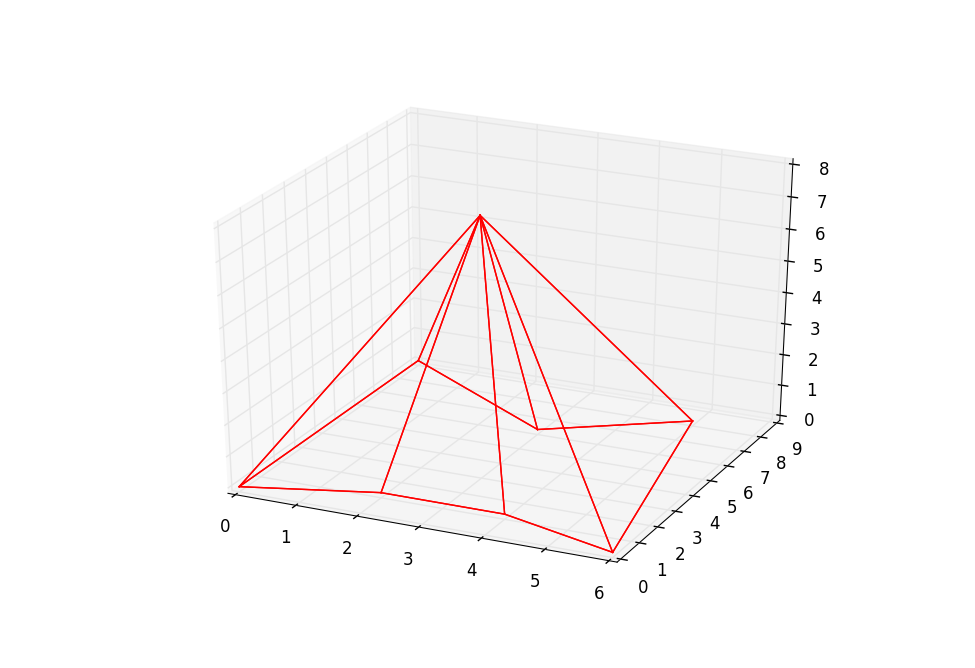
\includegraphics[scale=0.4]{images/matplotlibTest5.png}
\caption{Plot with Matplotlib. A specific mesh element that VEM can handle.}\label{img:geom}
\end{figure}

Then Figure \ref{img:matplotlibMesh} shows a particular case of a cubic mesh in $3$D. This image has been generated using the script \verb|plotMesh|. 

In Figure \ref{img:mayavi2D}, we can see the solution using linear VEM of the following differential problem:
\begin{equation*}
\begin{cases}
-\Delta u = \frac{\pi^2}{2}\cos\left(\frac{\pi x}{2}\right)\cos\left(\frac{\pi y}{2}\right) \text{ in } \Omega=(-1,1)^2;\\
u = 0 \text{ on } \partial \Omega,
\end{cases}
\end{equation*}
whose exact solution is $u(x,y)=\cos\left(\frac{\pi x}{2}\right)\cos\left(\frac{\pi y}{2}\right)$, for all $(x,y)\in \Omega=(-1,1)^2$. A rectangular mesh has been used to obtain this result. 

\begin{figure}[!h]
\centering
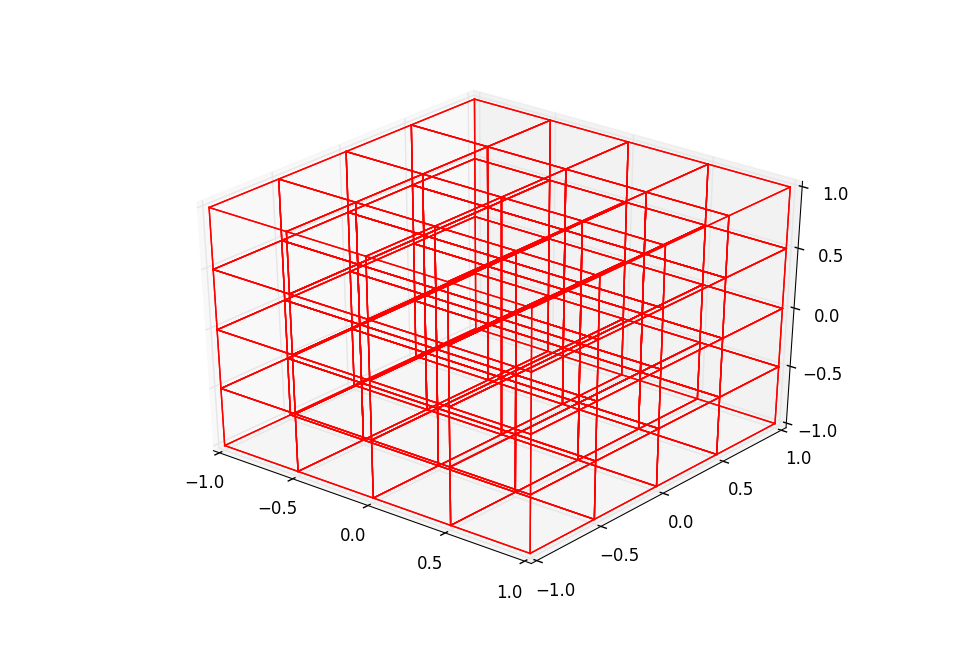
\includegraphics[scale=0.4]{images/matplotlibPlotMesh.png}
\caption{Plot with Matplotlib. Cubic mesh.}
\label{img:matplotlibMesh}
\end{figure}

\begin{figure}[!h]
\centering
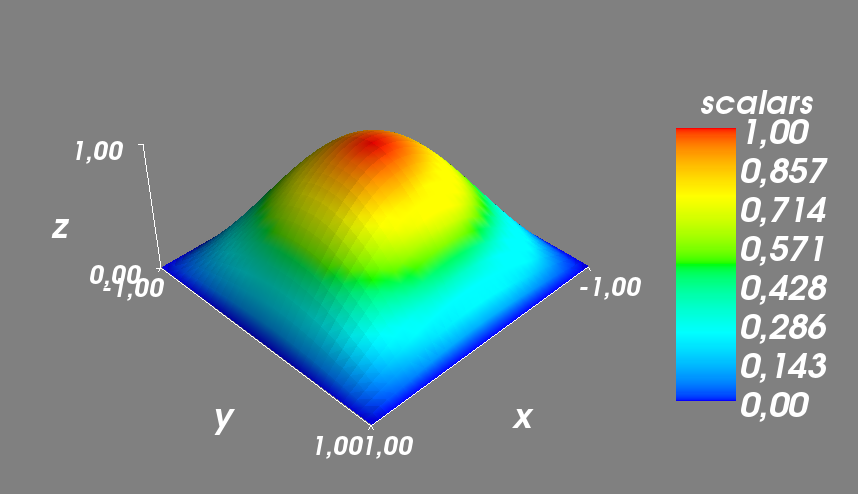
\includegraphics[scale=0.35]{images/mayavi2D.png}
\caption{Plot with Mayavi. VEM solution on a $2$D grid mesh.}
\label{img:mayavi2D}
\end{figure}

Figures \ref{img:mayaviCoupe} and \ref{img:mayavi3D} show the solution using linear VEM of the following differential problem:
\begin{equation*}
\begin{cases}
-\Delta u = 6 \text{ in } \Omega=(0,1)\times (0,2\pi) \times (0,\pi).\\
u = 0 \text{ on } \partial \Omega,
\end{cases}
\end{equation*}
where everything is expressed in spherical coordinates $(r,\phi,\theta)$, including Laplace operator. The exact solution is $u(r,\phi,\theta)=1-r^2$, for all $(r,\phi,\theta)\in (0,1)\times (0,2\pi) \times (0,\pi)$. Figure \ref{img:mayaviCoupe} shows only the solution on a section of the sphere while in Figure \ref{img:mayavi3D}, we can see the results on each vertex of the mesh. The size of the vertices and their color both correspond to the value of the solution on them. 

\begin{figure}[!h]
\centering
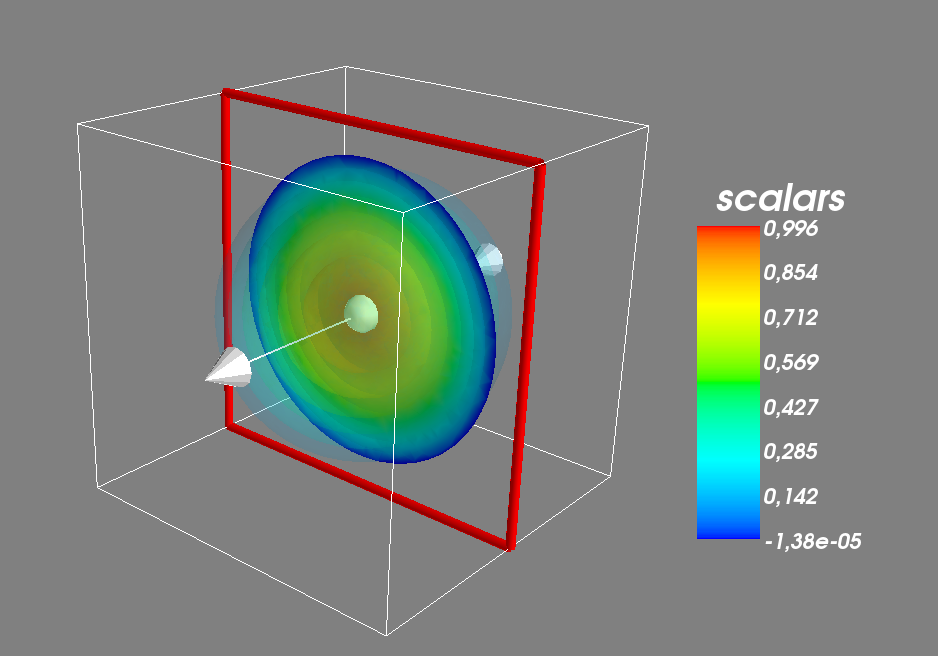
\includegraphics[scale=0.35]{images/mayavi3D.png}
\caption{Plot with Mayavi. VEM solution on a section of a $3$D sphere, with a mesh made of tetrahedra. The section can be dynamically chosen.}
\label{img:mayaviCoupe}
\end{figure}

\begin{figure}[!h]
\centering
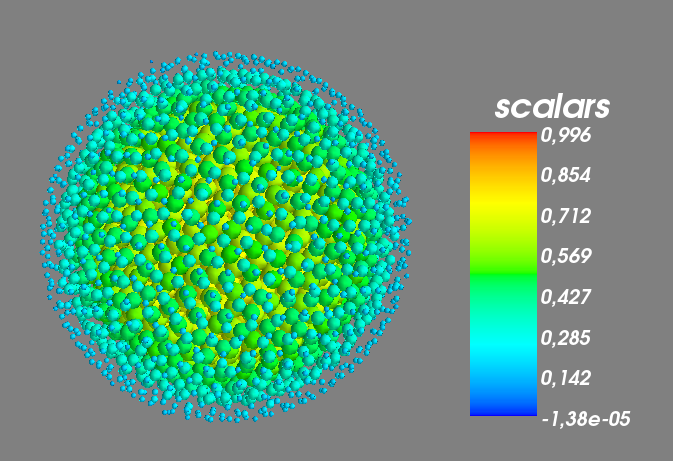
\includegraphics[scale=0.35]{images/mayavi3DPoints.png}
\caption{Plot with Mayavi. VEM solution on every vertex of a $3$D sphere, with a mesh made of tetrahedra.}
\label{img:mayavi3D}
\end{figure}

\subsection{Numerical results}

In this section, we will analyse numerically the convergence under $h$-refinement (that is when the mesh is refined) of the absolute a priori $H^1$-error of the solution, i.e. $\|u_h-u_{\text{ex}}\|_{H^1(\Omega)}$. $u_h$ is the solution found with the linear Virtual Element Method while $u_{\text{ex}}$ is the exact solution. Some particular differential problem will be analysed and presented behind.\\

Let $\Omega$ be the full sphere centered in $(0,0,0)$ and of radius $1$. Consider a mesh decomposition and let $h$ be the maximum diameter of the elements of this mesh. The considered meshes can be found in the folder \verb!Mesh/Sphere3D/!. We will analyse the $3$D behaviour of the error when we solve the following problem, expressed in spherical coordinates: find $u$ such that 
\begin{equation*}
\begin{cases}
-\Delta u = 6 \text{ in } \Omega = (0,1)^2;\\
u = 0 \text{ on } \partial \Omega.
\end{cases}
\end{equation*}
The exact solution of this problem is $u(r,\phi,\theta)=1-r^2$, for all $(r,\phi,\theta)\in\Omega$. \\

In Figure \ref{img:convSphere} is plotted the absolute a priori error in $H^1(\Omega)$-norm. We can clearly see that asymptotically, the error behaves as $h$, which is what one could expect after reading Theorem \ref{conditions} and section \ref{errors}. 

\begin{figure}[!h]
\centering
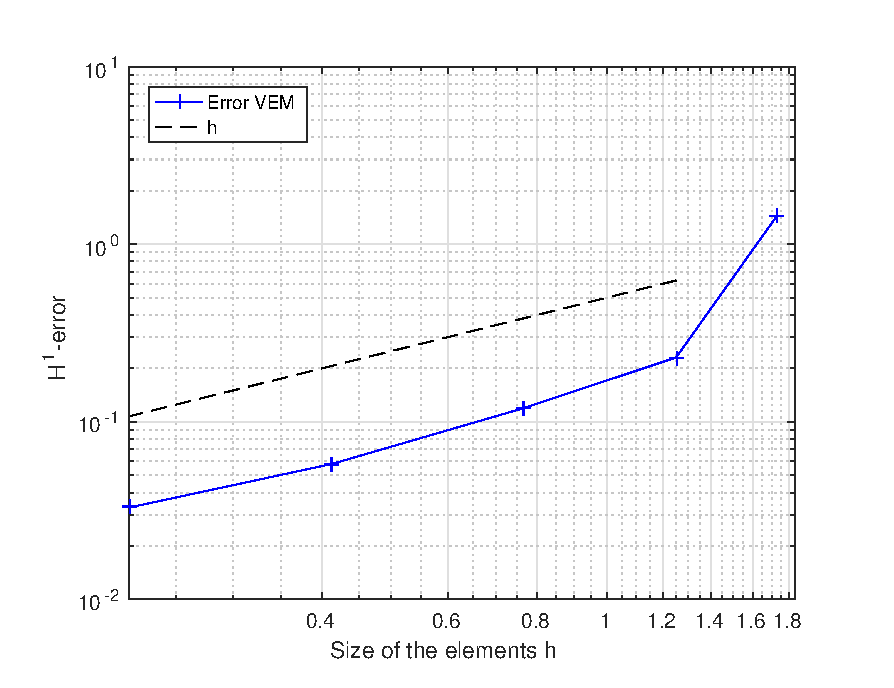
\includegraphics[scale=0.8]{images/convergenceSpherePlot3D.eps}
\caption{Convergence of the $H^1$-error under $h$-refinement for Laplace 3D problem on the sphere centered in $(0,0,0)$ and of radius $1$, with homogeneous Dirichlet boundary conditions.}
\label{img:convSphere}
\end{figure}

This behaviour is again confirmed when computing the slope of the log-log scale line. Indeed, we suppose that err $:=\|u_h-u_\text{ex}\|_{H^1(\Omega)} = Ch^p$, where $C$ is a constant depending only on the solution and on $k$, the degree of the underlying polynomials, which is here $1$. Our aim is to find $p$, so that we compute 
\begin{equation}\label{ploglog}
\frac{\log\left(\frac{\text{err}(h_2)}{\text{err}(h_1)}\right)}{\log\left(\frac{h_2}{h_1}\right)}=p,
\end{equation}
where err$(h_1)$ and err$(h_2)$ are the absolute a priori errors using a mesh size equal to $h_1$ and $h_2$, respectively. The values of the $p$ found thanks to the last $4$ points of Figure \ref{img:convSphere} are reported in the following Table \ref{tableSphere} and confirm our hypothesis. \\

\begin{table}[h!]
\begin{center}
\begin{tabular}{|c|c|c|}
\hline
$h_1$ & $h_2$ & $p$ \\
\hline
$1.2502$ & $0.7646$ & $1.3371$\\
\hline
$0.7646$ & $0.4134$ & $1.1726$\\
\hline
$0.4134$ & $0.2160$ & $0.8667$\\
\hline
\end{tabular}
\end{center}
\caption{Sum up of the convergence rates under h-refinement, on Laplace $2$D problem.} \label{tableSphere}
\end{table}

Furthermore, we have remarked that in the case of a very regular mesh composed of always equal simple convex polygons, we obtain a quadratic convergence, both in $2$D and in $3$D. Here are presented two examples of such phenomenon, one in $2$D and one in $3$D. 
In the following, we will only consider a decomposition of the space into identical elements, so
that we can define $h$ as the size of the elements. More precisely, we only consider squared or cubic elements, respectively for a $2$D or a $3$D problem, so that $h$ is the length of each side of each element.
Moreover, we will consider the geometry $\Omega=(0,1)^d$, where $d=2$ in the $2$D case, and $d=3$ in the $3$D case. Then $h=\frac{1}{n_e}$, where $n_e$ is the number of elements used on each direction. We have chosen to consider $n_e=1, 2, 4, 8, 16, 32, 64$ and $128$ elements, that is $h$ ranges from $1$ to $\frac{1}{128}$. $n_e$ is chosen as a sequence of powers of $2$ in order to have embedded spaces when the number of elements is increased.\\

First, we will analyse the $2$D behaviour of the error when we solve the following problem: find $u$ such that
\begin{equation*}
\begin{cases}
-\Delta u = 98\pi^2\sin(7\pi x)\sin(7\pi y) \text{ in } \Omega = (0,1)^2;\\
u = 0 \text{ on } \partial \Omega.
\end{cases}
\end{equation*}
The exact solution of this problem is $u(x,y)=\sin(7\pi x)\sin(7\pi y)$, for all $(x,y)\in \Omega$. This problem has been chosen so that the error between the numerical and the exact solution is large, since the solution oscillates a lot. In this way, the behaviour of the error can more easily be observed, since there is no risk to attain the machine epsilon too early. \\

In Figure \ref{img:conv2d} is plotted the absolute a priori error in $H^1(\Omega)$-norm. We can clearly see that asymptotically, the error behaves as $h^2$, which is one order of magnitude more than what one could expect from Theorem \ref{conditions}. It does not mean that the theorem is wrong, it just mean that the estimation is pessimistic is some cases such as this one, when the mesh is composed of regular and simple polygonal elements. 

\begin{figure}[!h]
\centering
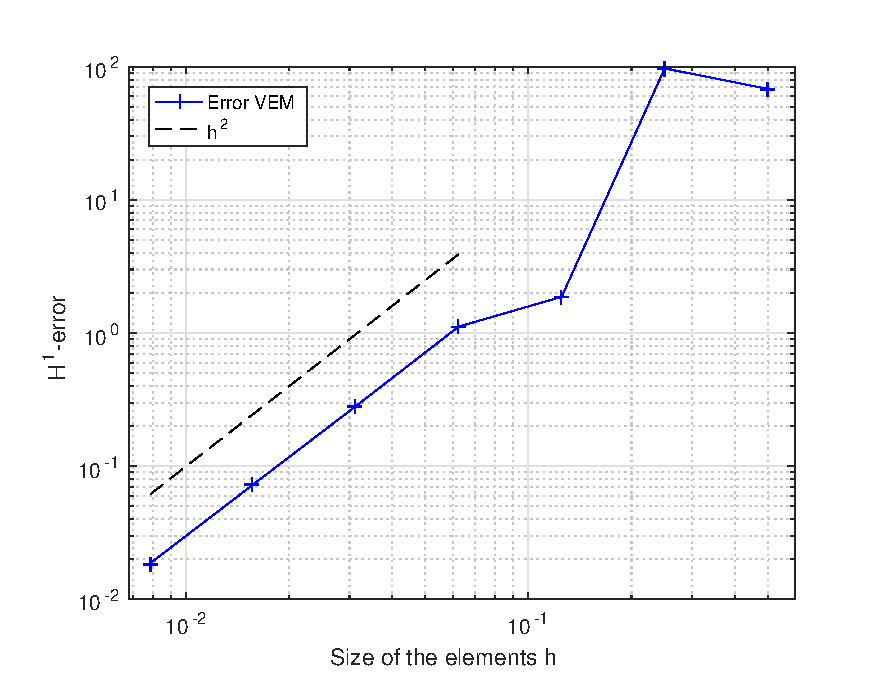
\includegraphics[scale=0.8]{images/convergencePlot2D.eps}
\caption{Convergence of the $H^1$-error under $h$-refinement for Laplace 2D problem on $(0,1)^2$ with homogeneous Dirichlet boundary conditions.}
\label{img:conv2d}
\end{figure}
This behaviour is again confirmed when computing the slope of the log-log scale line. The values of the $p$ found thanks to the last $4$ points of Figure \ref{img:conv2d} are reported in the following Table \ref{tableRect} and confirm our hypothesis.
\begin{table}[h!]
\begin{center}
\begin{tabular}{|c|c|c|}
\hline
$h_1$ & $h_2$ & $p$ \\
\hline
$16^{-1}$ & $32^{-1}$ & $1.9884$\\
\hline
$32^{-1}$ & $64^{-1}$ & $1.9612$\\
\hline
$64^{-1}$ & $128^{-1}$ & $1.9651$\\
\hline
\end{tabular}
\end{center}
\caption{Sum up of the convergence rates under h-refinement, on Laplace $2$D problem, with a very regular rectangular mesh.} \label{tableRect}
\end{table}
Finally, the non asymptotic behaviour is more chaotic since the approximation is very raw with very few elements. Let us add that the same behaviour has been observed when taking $u_\text{ex}(x,y)=\exp(7xy)$ on $(0,1)^2$, so that it is not solution-specific.\\

Now, we analyse the $3$D behaviour of the error when we solve the following problem: find $u$ such that
\begin{equation*}
\begin{cases}
-\Delta u = 127\pi^2\sin(7\pi x)\sin(7\pi y)\sin(7\pi z) \text{ in } \Omega = (0,1)^3;\\
u = 0 \text{ on } \partial \Omega.
\end{cases}
\end{equation*}
The exact solution of this problem is $u(x,y,z)=\sin(7\pi x)\sin(7\pi y)\sin(7\pi z)$, $\forall (x,y,z)\in \Omega$. Again and for the same reason as before, this problem has been chosen so that the error between the numerical and the exact solution is large, since the solution oscillates a lot. \\

In Figure \ref{img:conv3d} is plotted the absolute a priori error in $H^1(\Omega)$-norm. We can see again that asymptotically, the error behaves as $h^2$, which is again one order of convergence more than what one could expect from Theorem \ref{conditions}. To see it in a clearer way, we should refine the mesh even more, but a lot of RAM is needed to solve the problem ($>32$GB). Indeed, with $h=128$, we already take into account $128^3>2$ million degrees of freedom. 

\begin{figure}[!h]
\centering
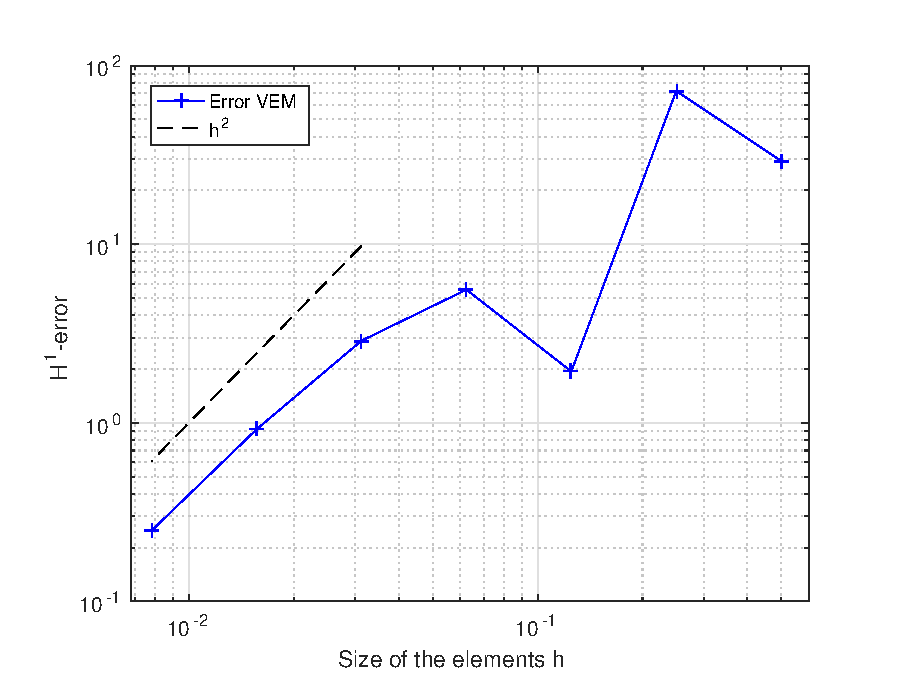
\includegraphics[scale=0.8]{images/convergencePlot3D.eps}
\caption{Convergence of the $H^1$-error under $h$-refinement for Laplace 3D problem on $(0,1)^3$ with homogeneous Dirichlet boundary conditions.}
\label{img:conv3d}
\end{figure}

Similarly as in the $2$D case, we can algebraically compute the slope of the log-log scale line to confirm our hypothesis, thanks to the same formula (\ref{ploglog}). The values of $p$ found thanks to the last $3$ points of Figure \ref{img:conv3d} are reported in the following Table \ref{tableCube} and indeed confirm the behaviour.
\begin{table}[h!]
\begin{center}
\begin{tabular}{|c|c|c|}
\hline
$h_1$ & $h_2$ & $p$ \\
\hline
$32^{-1}$ & $64^{-1}$ & $1.7497$\\
\hline
$64^{-1}$ & $128^{-1}$ & $1.9293$\\
\hline
\end{tabular}
\end{center}
\caption{Sum up of the convergence rates under h-refinement, on Laplace $3$D problem.} \label{tableCube}
\end{table}

Let us add that the same behaviour has been observed when taking $u_\text{ex}(x,y,z)=\exp(7xyz)$ on $(0,1)^3$, so that it is not solution-specific. 
Note moreover that this $h^2$-component of the error is a typical characteristic of finite element-type methods: the classical finite element methods \cite{quarteroni}, the spectral element methods \cite{chqz1}, the isogeometric analysis \cite{igaconv}.


%Section Conclusion
\newpage
\section{Conclusion}

TODO
%Section Appendix : TODO add or not?
%\newpage
\section{Appendix}

TODO
In this section, we will give some results that we use in other sections. Generally, these are well-known results.


\vfill

%Référence et bibliographie :
\begin{thebibliography}{99}
\bibitem{existenceW} Ahmed B., Alsaedi A., Brezzi F., Marini L.D., Russo A., \textit{Equivalent projectors for virtual element methods}, Comput. Math. Appl., 66 (2013) 376-391.
\bibitem{hitchhicker} Beirão da Veiga L., Brezzi F., Marini L.D., Russo A., \textit{The Hitchhiker's Guide to the Virtual Element Method}, Mathematical Models and Methods in Applied Sciences, 24 (8) 1541-1573, 2014.
\bibitem{brennerscott} Brenner S.C., Scott R.L., \textit{The Mathematical Theory of Finite Element Methods}, Texts in Applied Mathematics, Vol. 15 Springer-Verlag, 2008.
\bibitem{basicpples} Beirão da Veiga L., Brezzi F., Cangiani A., Manzini G., Marini L.D., Russo A., \textit{Basic principles of virtual element methods}, Mathematical Models and Methods in Applied Sciences, 23 (1) 199-214, 2013.
\end{thebibliography}

\end{document}

%$$\begin{array}{ccccc}f&:&L&\longrightarrow &L\\&&y&\longmapsto &z\end{array}$$